\documentclass[dissertation, copyright, numbers, sort&compress, notables]{uothesis}

\usepackage[english]{babel}
\usepackage{graphicx}
\usepackage{dcolumn}% Align table columns on decimal point
\usepackage{bm}% bold math
\usepackage{float}
\usepackage{physics} %bra-ket
\usepackage{amsmath}
\usepackage{amsfonts}
\usepackage{amssymb}
\usepackage{color}
\usepackage{placeins}
\usepackage{url}
\usepackage{dcolumn}% Align table columns on decimal point
\usepackage{bm}% bold mathu
\usepackage[noabbrev]{cleveref}

%\usepackage[justification=justified]{subcaption} 

\usepackage[dvipsnames]{xcolor}
\newcommand{\be}{\begin{equation}}
\newcommand{\ee}{\end{equation}}
\newcommand{\of}[1]{\left(#1\right)}
\newcommand{\pd}{\partial}

\newcommand{\eps}{\varepsilon}
\newcommand{\utot}{U}
\newcommand{\mpv}{\bar{V}_{\mathrm{p}}} %mean particle volume

%????????????????
%\DeclareUnicodeCharacter{2009}{\,} 

\newcommand{\ec}[1]
{\textcolor{red}{#1}}

\definecolor{mygray}{gray}{0.4}
\newcommand{\greytext}[1]
{\textcolor{mygray}{#1}}

\newcommand{\jamesemph}[1]
{\textcolor{blue}{#1}}


%%%PREFATORY PAGES
\covertitle{TITLE HERE}
\abstracttitle{ABSTRACT TITLE HERE}
\author{James Sartor}
\department{Department of Physics}
\narrowdepartment{Department of Physics}
\degreetype{Doctor of Philosophy}
\degreemonth{December}
\degreeyear{2021}

\advisor{Eric Corwin}
\chair{Ben Mcmorran}
\committee{Jayson Paulose &  Core Member\\
Marina Guenza &  Institutional Representative\\}
\graddean{Andy Karduna}

\abstract{
abstract here
%A vast variety of physical systems falls within the description of amorphous solids. From glasses to grains, all of these materials share a disordered structure of their constituents. Understanding the nature of the mechanical properties of such systems is a conundrum which still poses challenging open questions. Recent experimental advances have led to the conclusion that the preparation of the system controls its stability against mechanical perturbations. In particular, amorphous solids can be classified as marginally stable or highly stable with respect to external perturbations. In this work I show that the amorphous structure, whether marginally or highly stable, uniquely controls the mechanical response of amorphous solids. First, I show that thermal glasses under very high pressure share the same mechanical and vibrational properties of athermal granular packings near the onset of rigidity. Secondly, I investigate the role of mechanical stability in the context of rheology, in particular with respect to cyclic shear training, and show that jammed solids are able to store an information of the repeated shear deformation only if the system, or a portion of it, is marginally stable.

This dissertation includes previously published and unpublished coauthored material.}

\acknowledge{
Full acknowledgement of all the support I've received through the writing of this would be longer than the dissertation itself. Nevertheless, I'd like to take a moment to express my gratitude here to those who have contributed the most to this work.

First and foremost I would like to thank my advisor Eric Corwin for his unwavering support over the past five years. Without your enthusiasm, expertise, and flexibility, this would not have been possible.

I am grateful as well for the excellent labmates that I have had here, for myriads of help and support: Cam Dennis, Francesco Arceri, Varda Faghir Hagh, Andy Hammond, Valerie Beale, Aileen Carroll-Godfrey, Jack Dale, Jacob Hass, Alex Trevelyan, Georgios Tsekenis, and Mike van der Naald. 

Special thanks to Sean Ridout for not only the contributions to the letter which we wrote together, but also for providing insightful feedback on my other projects. 
I would also like to acknowledge Francesco Zamponi for graciously elucidating mean field results for us.

Thanks to Peter Morse for advice on both research and death cults. I would also like to acknowledge my committee for their advice and support throughout this process.

Lastly I would like to thank all my friends and family for their support, as well as innumerable fellow grad students, faculty, and staff who have helped me in various ways through this time.

This work was supported by the NSF Career Award grant No. DMR-1255370, and the Simons Collaboration on Cracking the Glass Problem (No. 454939 E. Corwin)}
  %%acknowledgements page optional
\school{University of Oregon, Eugene, OR, USA}
\school{University of La Sapienza, Rome, ITALY}

\degree{Doctor of Philosophy, Physics, 2021, University of Oregon}

\degree{Master of Science, Physics, 2017, University of La Sapienza}

\degree{Bachelor of Science, Department of Physics, Physics, 2014, University of La Sapienza}

%%There is a known issue if you do not fill in the interests section.  If you want to skip this section, comment out line#526 of uothesis.cls file \cvitem{AWARDS AND HONORS}{\@awards}
\interests{Soft Condensed Matter, Jamming, Rheology, Active Matter}

\position{Research Assistant, University of Oregon, 2019-2021}
\position{Teaching Assistant, University of Oregon 2017-19}

%%\award{[Award, Project Title, Institution, Year]}
\award{Weiser Senior Teaching Assistant Award, UO Department of Physics, 2019}
\award{Weiser First Year Teaching Assistant Award, UO Department of Physics, 2018}

\publication{ F. Arceri, E. I. Corwin, and Varda F. Hagh, ``Marginal Stability Enables Memory Training in Jammed Solids" {\sl arXiv preprint} arXiv:2106.05442 (2021)}
\publication{ F. Arceri, and E.I. Corwin, ``Vibrational properties of hard and soft spheres are unified at jamming" {\sl Phys Rev Letters }  \textbf{112} (23) 238002 (2020).}
\publication{ F. Arceri, L. Berthier, G. Biroli, and F. Landes, ``Glasses and aging: a statical mechanics perspective" {\sl arXiv preprint} arXiv:2006.09725 (2020).}

%\include{dedication} %%dedication page optional

%%%MAIN DOCUMENT
\begin{document}
\maketitle

here is some text
%%%CHAPTERS
%\chapter{Introduction}

%When you think of solids, you generally think of crystals. You take a liquid, and let it cool down, and it falls into a nice crystal structure that is spatially optimized in some way. This is generally how most solids form and is conceptually pretty easy to understand. Glass however can be formed by cooling down a liquid too quickly to find its minimum energy configuration - it essentially just gets stuck in some non-optimal state instead. 

Anyone who has stacked oranges knows that it is easy and intuitive to stack them closely in a dense lattice, as demonstrated in figure \ref{plot:oranges}(a). Filling about $74\%$ of space, the close packed lattice is in fact the densest possible arrangement of equal sized spheres in 3 dimensions. This was originally conjectured by Kepler in 1611 \cite{kepler_strena_1611}, but was not formally proven until 1998 \cite{hales_overview_1998}. If one simply pours them together, they will instead arrange themselves in an amorphous (i.e. random) and less dense structure, as shown in figure \ref{plot:oranges}(b). This amorphous configuration is significantly less efficient, filling only $0.62\%$ of space. The lazy but innovative produce worker may attempt to create a close lattice by randomly pouring oranges into a box and squeezing, but experience dictates that this is impossible. The fruit are too much in each other's way to rearrange and relieve the stress from the squeezing. Interestingly, 2 dimensional discs of equal size do spontanously form hexagonal lattices when squeezed, but discs of nonuniform size generally become frustrated and arrange amorphously.

\begin{figure}[b!]

\includegraphics[width=\columnwidth, trim=0 0 0 0, clip]{oranges.pdf}

\caption{Left, stack of oranges constructed in a close packed lattice. Right, oranges arranged amorphously. \jamesemph{[how to cite these appropriately?]}}
%https://unsplash.com/photos/A4BBdJQu2co
%https://www.tate.org.uk/art/artworks/louw-soul-city-pyramid-of-oranges-t13881

\label{plot:oranges}
\end{figure}

Granular materials are collections of distinct macroscopic objects, such as sand, ball bearings, or piles of oranges. While crystalline structures such close lattices are relatively straightforward to understand and analyze, the random features of amorphous granular systems make them extremely difficult to understand from first principles. The only analytic approach that has been somewhat successful is by taking the limit of infinite spatial dimensions, termed ``mean field.'' Since all physical systems are finite dimensional, results from the mean field limit do not necessarily apply. Many results from the mean field are however surprisingly accurate even in as low as 2 and 3 dimensions. Our research is not focused on analytic theory, but rather on computational study of soft spheres, i.e. spheres which are able to interact with their neighbors, imparting variable forces upon them. %Although the forces between granules of physical systems arise from physical deformations, this can be approximated with non-deforming but slightly overlapping spheres. 
In general when we simulate systems in greater than three dimensions, the purpose is to draw parallels with results from the mean field.


A phase transition is when a material undergoes a discontinuous change in some property (the ``order parameter'') as some other property (the ``control parameter'') varies. The most well known phase changes are freezing/melting and boiling/condensating, for which the temperature is the control parameter, and the density of the material can be seen to discontinuously change at critical temperatures. The order parameter is generally accepted to be the free energy - at the phase transition, melting absorbs a latent heat separate from the heat required just to heat it to the melting point. While glasses go through thermal phase transitions, granular materials do not. Granular materials are thus described as being ``athermal'' or ``zero-temperature.'' If you imagine the box of oranges as described earlier, thermal fluctuations (providing energy $E \sim kT \sim 0.026$ eV) will never cause rearrangements of a pair of oranges (requiring $E \sim mgr \sim 10^{17}$ eV). Granular materials do however go through a different type of transition, called the jamming and unjamming transitions, which are somewhat analogous to thermodynamic phase transitions. The control parameter for the jamming transition is the density $\varphi$, and the jamming transition happens at a critical density $\varphi_j$, where properties of the system go through discontinuous changes. In particular, the pressure $P$ goes from 0 to a finite value, and the number of force bearing contacts between granules goes from 0 to roughly the number of particles times the spatial dimension $Nd$. The critical density is an exact value for any particular system, but generally has some variation between systems, and can vary based on the protocol of system generation. The jamming point can be understood as a critical point, and as the system increases in density from that point, properties such as the number of contacts in excess of Nd, the pressure, and the density in excess of $\varphi_j$ all scale with each other as power laws \cite{ohern_jamming_2003,goodrich_scaling_2016}.

Traditional approaches to analyzing thermodynamic systems rely on the assumption of ergodicity, i.e. that the thermal system explores the ensemble of all available configurations. The probability of existing in any particualar configuration is related to the energy of that configuration compared with the temperature of the system. In a zero temperature granular material, however, this is obviously impossible. Despite this, granular materials respond predictably to repeated disturbances, e.g. if you repeatedly shake a box of rocks, they will reliably settle into a configuration of roughly the same density. Thus some version of athermal statistical mechanics is clearly at work. In 1989 Sir Sam Edwards begun the first serious attempt at understanding granular materials in thermodynamic terms \cite{edwards_theory_1989}. The parameters compactivity and angoricity arose as granular analogs to temperature that relate to density and pressure respectively rather than temperature. While this approach has had some success, measurement of angoricity and compactivity is difficult \jamesemph{[re-read this review and write something more meaningful here lol]} \cite{bi_statistical_2015}.

The jamming transition describes the onset of rigidity. Below $\varphi_j$, a system is floppy and unable to sustain any force. Above $\varphi_j$ however a system becomes rigid and can support external forces. You can run your hands through sand at the beach, but if you compress it, it will push back. This rigidity can be understood in terms of degrees of freedom and constaints - it arises when the system has at least as many constraints as degrees of freedom. A system where these are exactly equal is termed ``isostatic,'' and a system with more constraints than degrees of freedom is termed ``hyperstatic.'' Since each particle can move in $d$ dimensions, a granular system has $Nd$ degrees of freedom. The constraints on those degrees of freedom are the contacts between particles, which increase in quantity with increasing density or pressure. The jammed configurations that we study are hyperstatic and thus are rigid and may support external forces. When considering instead the force network of the system, each contact is a degree of freedom, and requiring force balance on each particle imposes $Nd$ constraints. Thus while the positions of particles in a hyperstatic system is overdetermined, the force network supporting this rigidity is underdetermined. There exists a degerate space of allowed force configurations, which is referred to as the Force Network Ensemble or FNE \cite{snoeijer_force_2004,tighe_force_2010}. \jamesemph{[something about how we use it]}

The following three chapters are the three papers which we composed during my time as a graduate student. The first explores a method that we developed that uses the Force Network Ensemble to measure the allowed space of force configurations. This allowed us to measure the angoricity and thus the entropy of the force networks of a granular system. In the second, we use a similar approach to examine the boundaries of the allowed space of force configurations. These boundaries correspond to systems with fewer contacts than the original system. By examining which contacts are missing in those systems, we are able to predict which contacts between particles are unnecessary. We then show that these contacts are in fact broken under decompression. In the third, we closely examine the relation between a few critical power laws from the jamming transition. Rather than looking at the well known exponents of these power laws, we explore the prefactors to these power laws. Although pefactors such as these are generally highly sensitive to finite dimensional corrections, we show that they are still well predicted by the mean field.


\chapter{Direct measurement of force configurational entropy in jamming}
\author{James D Sartor, Eric I Corwin}
%\affiliation{Department of Physics and Materials Science Institute, University of Oregon, Eugene, Oregon 97403, USA}
%\date{\today}

\label{forceVolumeEntropyPaper}

%\begin{abstract}


\section{Abstract}
Thermal fluctuations are not large enough to lead to state changes in granular materials. However, in many cases, such materials do achieve reproducible bulk properties, suggesting that they are controlled by an underlying statistical mechanics analogous to thermodynamics.
While themodynamic descriptions of granular materials have been explored, they have not yet been concretely connected to their underlying statistical mechanics.
We make this connection concrete by providing a first principles derivation of the multiplicity and thus the entropy of the force networks in granular packings. 
We directly measure the multiplicity of force networks using a protocol based on the phase space volume of allowed force configurations.
Analogous to Planck's constant, we find a scale factor, $h_f$, that discretizes this phase space volume into a multiplicity.
To determine this scale factor, we measure angoricity over a wide range of pressures using the method of overlapping histograms and find that in the absence of a fundamental quantum scale it is set solely by the system size and dimensionality. This concretely links thermodynamic approaches of angoricity with the microscopic multiplicity of the force network ensemble.
%\end{abstract}



\section{Introduction}
Thermodynamics connects abstract and difficult to measure details, such as entropy, with more easily measured bulk properties, such as temperature. In granular systems, for which the thermal energy scale is irrelevantly small, similar connections have been proposed for the volume ensemble \cite{edwards_theory_1989,bi_statistical_2015} using compactivity as a temperature analog and also for the force network ensemble \cite{edwards_distribution_2008, bi_statistical_2015} using angoricity. 
While these quantities are measurable \cite{puckett_equilibrating_2013,bililign_protocol_2019}, they are not physically meaningful unless they 1) are shown to have temperature-like properties, such as following the zeroth law and 2) can be rigorously linked to a first principles definition of microscopic entropy~\cite{grimus_100th_2013}. 
Entropy itself was initially an empirical quantity until Sackur and Tetrode placed it on firm footing for the ideal gas with the discretization of phase space into quantum mechanical states \cite{tetrode_chemische_1912,grimus_100th_2013}. The length scale of the discretization depends both on properties of the system and the universal constant $\hbar$, whose value cannot be inferred from bulk properties of the ideal gas alone.
Angoricity holds promise as a temperature analog, as it has been shown to follow the zeroth law, while compactivity fails to do so \cite{bi_statistical_2015, puckett_equilibrating_2013,edwards_granular_2002}. However, before the thermodynamic approach of angoricity can be considered to be on solid ground, the nature of the entropy of jammed systems must first be understood. 

When the density of an overjammed packing increases, force networks are affected in two ways: 1) force magnitudes, and thus pressure, increase, and 2) new contacts between particles form, increasing the number of contact forces in the network. Both of these changes increase the entropy of the force networks. While the effect on entropy from  pressure changes is well understood \cite{bililign_protocol_2019,henkes_statistical_2009}, the effect from changes in the contact network is not. To decouple these effects, we propose an extension to the Force Network Ensemble in which changes in the contact network are allowed. This leads us to identify a critical number of excess contacts, $\delta z_c$, describing the transition from a regime in which entropy is dominated by changes in pressure to one in which it is dominated by changes in the contact network.

The temperature analogue angoricity is defined as the derivative of entropy with respect to the stress tensor
\cite{edwards_distribution_2008}. In isotropic systems this tensor quantity can be simplified to a scalar derivative of entropy with respect to pressure. Just as temperature of an ideal gas can be measured from the velocity distribution, angoricity can be measured from the distribution of local pressures \cite{bililign_protocol_2019}. As a derivative, angoricity provides information about the difference in entropy between two systems but not the absolute values. Previous theoretical and experimental work has identified an inverse scaling of angoricity with pressure in the near jamming limit for two-dimensional (2D) soft spheres \cite{henkes_statistical_2009,bililign_protocol_2019}. However, these studies do not systematically explore the effect of changing the contact network, which remains static in the near jamming limit. In our computational study, we explore the system by varying the spatial dimension, pressure, and number of particles over ranges much larger than would be feasible in a physical experiment.

In this Rapid Communication, we present a first principles derivation of the entropy for the force networks of granular packings.  We measure this entropy up to a multiplicative constant, $h_f$, in the near jamming limit by directly measuring the volume of the space of allowed force configurations.  Analogous to Planck's constant in the Sackur-Tetrode equation, $h_f$ discretizes the space of force configurations into an integer number of accessible states.  We then use the method of overlapping histograms to measure angoricity as a function of pressure, and compare with our force volume measure to solve for $h_f$. This concretely connects the bulk nature of angoricity with the microscopic multiplicity of the force network ensemble.

\begin{figure*}[t]
\centering
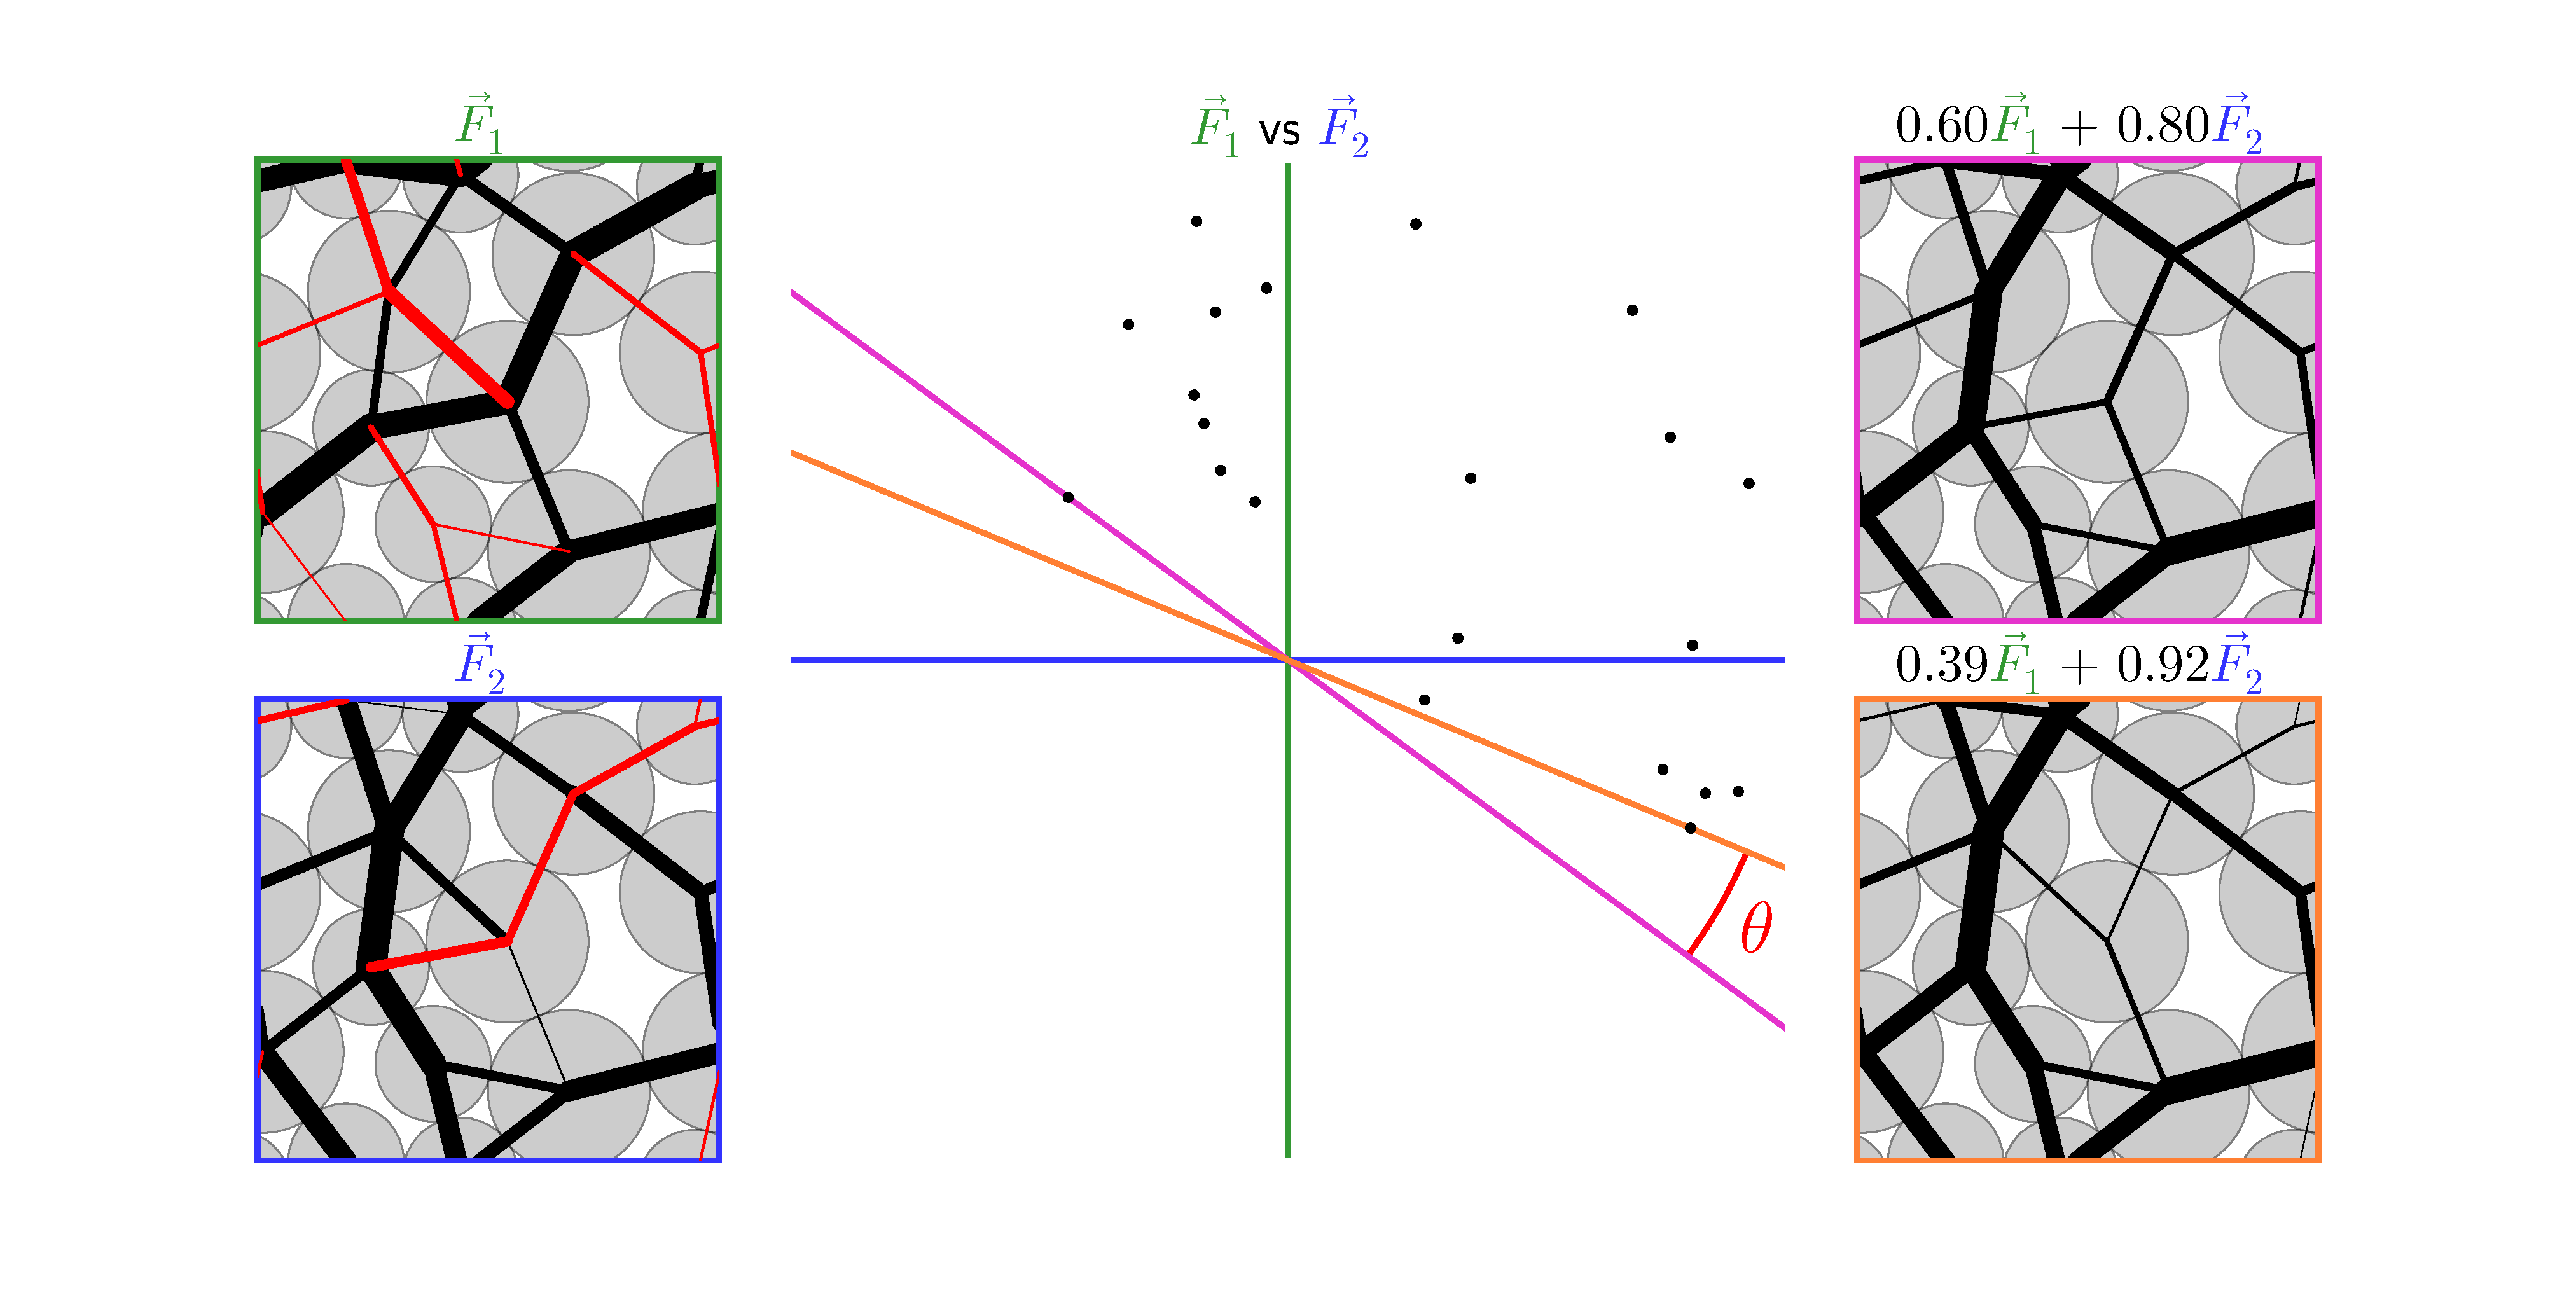
\includegraphics[width=\textwidth, trim=150 70 150 70, clip]{forceVolumeEntropyPaper/methodIllustration.pdf}
\caption{Force volume measurement for a system with one excess contact. Left, the two independent states of self stress, $F_1$ and $F_2$. Black lines between particles represent positive (compressive) forces, red lines represent negative (tensile) forces. 
Center, a scatter plot of $F_1$ vs $F_2$ for each pair of particles. Linear combinations of $F_1$ and $F_2$ are represented graphically by drawing a sloped line through the origin and measuring the distance to each point.  Any sloped line for which all of the points fall into the same half-space corresponds to a positive definite linear combination. The set of lines which allow for such solutions is the force space volume, indicated by the angle $\theta$. Note that in a system with $\Delta Z$ excess contacts, this volume is a $\Delta Z$ dimensional quantity.
Right, the two extremal positive-definite linear combinations at the edge of this region are shown. Each has one force brought to precisely zero.}
\label{methodIllustrationFigure}
\end{figure*}

 \section{Computational methods} We use pyCudaPacking \cite{charbonneau_universal_2012}, a GPU-based simulation engine, to generate energy minimized soft sphere packings at specified pressures in periodic boundary conditions. We do so for number of particles, $N$, spanning from 256 to 4096, and dimension, $d$, from 2 to 5. The particles are monodispersed, except in 2D in which we use equal numbers of bidispersed particles at a size ratio of 1.4:1 to prevent crystallization. Particles interact through a harmonic contact potential as defined in \cite{charbonneau_universal_2012}, and the system's energy is minimized using the FIRE minimization algorithm \cite{bitzek_structural_2006}.
 
Starting with random initial positions, we minimize energy and then adjust overall density by uniformly scaling particle radii to achieve a pressure $P$ of $10^{-2}$ in natural units, as defined in \cite{ohern_jamming_2003}. This pressure is chosen to prevent crystallization artifacts from high density packings. From there, we iteratively adjust the density both up and down to achieve specific values of pressure.  We do this efficiently by exploiting the known linear scaling of pressure with density above jamming for a harmonic potential \cite{goodrich_scaling_2016}. For each targeted pressure, we ensure that the actual pressure is accurate to a factor of $10^{-5}$. We sample 100 logarithmically spaced steps per decade of pressure to ensure sufficient overlap between the distributions of local pressure for neighboring systems, as is needed for the method of overlapping histograms.

\section{Rigidity}
To understand the behavior of packings close to the jamming transition we examine the geometric mechanisms necessary for rigidity by constructing an unstressed spring network with the geometry of the packing. The rigidity matrix \cite{charbonneau_jamming_2015, ellenbroek_rigidity_2015, f._hagh_broader_2019}, $\mathcal{R}$, describes this spring network by encoding the normalized contact force vectors from the packing, $n_{i j}$, between pairs of particles $i$ and $j$ as
%
\begin{equation}
    \mathcal{R}^{k \alpha }_{\left<ij\right>}=(\delta_{jk}-\delta_{ik}) n^\alpha_{ij},
\end{equation}
%
 where $k$ indexes contacts and $\alpha$ indexes spatial dimensions. For a system with $N_\textrm{stable}$ stable particles and $N_\textrm{contact}$ contacts, this will be an $N_\textrm{contact}$ by $N_\textrm{stable}d$ matrix.  The singular value decomposition of this matrix yields two sets of singular vectors, analogous to eigenvectors for a square matrix. The right singular vectors describe the normal modes of position displacements, and the left singular vectors describe the normal modes of force displacements. 
The left singular vectors corresponding to zero eigenvalues represent mechanically stable force configurations, termed states of self stress.
These vectors need not be positive definite, and therefore are not necessarily valid force configurations for the underlying packing.
 
The magnitude of each contact force can be considered as a degree of freedom while the requirement for mechanical stability introduces $d$ constraints for each particle.  Balancing these constraints requires a minimum number of contacts to ensure stability, which in systems with periodic boundary conditions is given by~\cite{dagois-bohy_soft-sphere_2012, goodrich_finite-size_2012}
 %
 \begin{equation}
     N^\textrm{min}_\textrm{contact} = d(N_\textrm{stable}-1)+1.
 \end{equation} 
 %
A system with this minimum number of contacts has exactly one state of self stress, and each additional contact formed imparts an additional independent state of self stress. Thus, we define the number of excess contacts, $\Delta Z$ as
 %
\begin{equation}
    \Delta Z=N_\textrm{contact}-N^\textrm{min}_\textrm{contact},
\end{equation}
 %
 making the number of independent states of self stress $\Delta Z+1$. We define the number of excess contacts per particle,
 %
 \begin{align}
 \delta z = 2\Delta Z / N,
 \end{align}
 %
where the 2 reflects that each excess contact is shared between two particles. These independent states of self stress form a basis for the $\Delta Z+1$ dimensional space of all mechanically stable force configurations of the spring network. However, imposing a normalization condition restricts this to a $\Delta Z$ dimensional subspace.

\section{Force Volume}
The force network ensemble samples all valid force networks in the spring representation of a packing with equal probability \cite{snoeijer_force_2004,tighe_force_2010,tighe_stress_2011}. 
To determine the force volume, we calculate the normalized independent states of self stress where $F_\mu^q$ is the contact force on contact $q$ in the state of self stress $\mu$.  The set of all possible repulsive contact forces is defined by linear combinations that satisfy
%
\begin{align}
\label{eqn:coefficientCondition}
\sum_\mu \lambda_\mu F_\mu^q \ge 0
\end{align}
%
for all contacts $q$, where $\{\lambda_\mu\}$ are coefficients subject to the normalization condition $\sum_\mu \lambda_\mu^2 = 1$.  We define the force volume $V_f$ to be the volume of the space of $\lambda_\mu$ coefficients that satisfy this rule as illustrated in Fig. \ref{methodIllustrationFigure}.  

We measure this force volume with the following protocol:
\begin{enumerate}
\item Recast $F_\mu^q$ into a set, $\{\vec{C}^q\}$, of $N_{\textrm{contacts}}$ vectors containing the value of the force on contact $q$ in each of the $\Delta Z+1$ states of self stress.
\item Planes which pass through the origin and place all of the $\{\vec{C}^q\}$ into a single half-space satisfy inequality (\ref{eqn:coefficientCondition}).  We compute the extremal values of such planes as the facets of the convex hull \cite{barber_quickhull_1996} of $\{\vec{C}^q, \vec{0}\}$.  The normal vector to each facet is the $\{\lambda_\mu \}$ which defines a vertex of the allowed space of coefficients and corresponds to a linear combination of the independent states of self stress in which exactly $\Delta Z$ forces are precisely 0.
\item To respect the normalization requirement we calculate $V_f$ as the $\Delta Z$ dimensional solid angle subtended by the volume defined by these vertices in coefficient space.
\end{enumerate}

We convert this volume into a pure number of configurations by discretizing it into hypercubes of side length $h_f$, named to emphasize the parallelism with Planck's constant $h$ used in the enumeration of phase space states in the Sackur-Tetrode equation.
Because the pressure sets the scale of the average force, we then multiply this enumeration by the pressure, as has been shown in previous theoretical and experimental work~\cite{henkes_statistical_2009,bililign_protocol_2019,mailman_using_2012}. Putting these considerations together, we arrive at an ansatz relating the microscopic force volume to the multiplicity, and thus the entropy:
%
\begin{align}
\Omega = P \frac{V_f}{(h_f)^{\Delta Z}} && \Longrightarrow && S=\ln P  + \ln{V_f} - \Delta Z \ln{h_f}.
\label{eqn:entropy}
\end{align}

Although pressure and number of excess contacts both appear in the entropy, they are not independent variables but related in the thermodynamic limit by~\cite{ohern_jamming_2003,goodrich_scaling_2016}
%
\begin{align}
\label{eqn:excess}
 \Delta Z = B(d) N \sqrt{P}.
\end{align}
%
where $B$ is some function of dimension only. We find values of $B$ of approximately 2.1, 6.0, 12.5, and 23 in dimensions two, three, four, and five. These values are roughly consistent with previous studies for two and three dimensional spheres \cite{ohern_jamming_2003, goodrich_finite-size_2012}. 

Angoricity~\cite{edwards_distribution_2008}, $\alpha$, is derived as:
%
\begin{align}
\label{eqn:angoricity}
\alpha &\equiv \frac{\partial S}{\partial P} = \frac{1}{P}  + \frac{\partial }{\partial P}\ln{V_f} - \frac{1}{2} \frac{BN}{\sqrt{P}}\ln{h_f}.
\end{align}
%
First, we measure the volume of force space $V_f$ and explore how it scales with the number of excess contacts. Second, we measure bulk angoricity to confirm our prediction in Eq. (\ref{eqn:angoricity}) and measure the microscopic constant $h_f$.

\begin{figure}[h!]
\centering
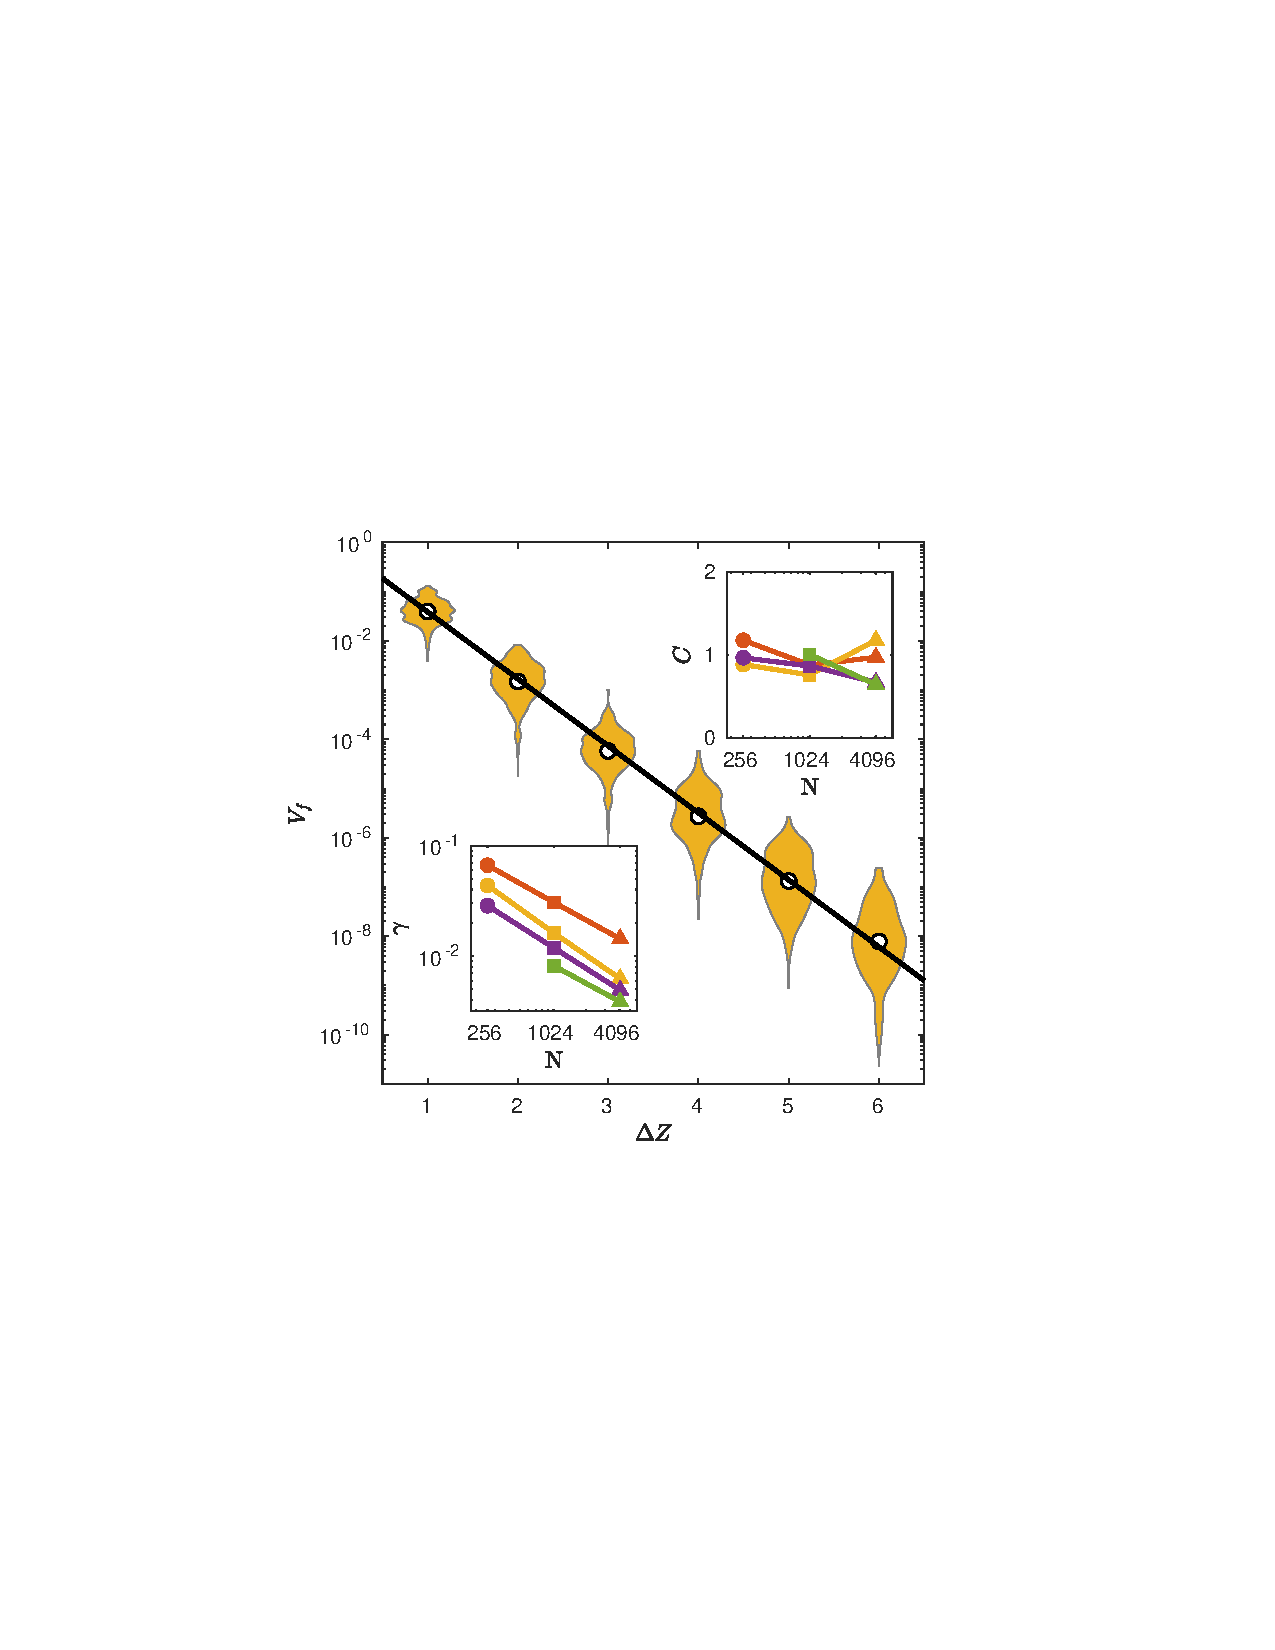
\includegraphics[width=\columnwidth, trim=137 240 165 254, clip]{forceVolumeEntropyPaper/volumeInset.pdf}
\caption{Representative exponential scaling of the force volume, $V_f$, with number of excess contacts, $\Delta Z$, for $N=1024$, $d=3$. The median of the distribution for each $\Delta Z$ is shown as a white circle, surrounded by the full distribution in yellow. The black line shows the exponential fitting form, with exponential base $\gamma$. Inset bottom left, $\gamma$ for each $N$ and $d$. Inset top right, the scale, $C$ of the exponential. Inset data is presented for $d$ = 2 (red), 3 (yellow), 4 (purple), and 5 (green), and $N$ = 256 (circles), 1024 (squares), and 4096 (triangles).}
\label{volumePlot}
\end{figure}

\section{Results}
As shown in Fig. \ref{volumePlot}, the measured force volume scales exponentially with the number of excess contacts:
%
\begin{align}
 \label{eqn:forceVolume}
 V_f~=~C\gamma ^ {\Delta Z}.
\end{align}
%
We find $C$ to be well approximated by $1$, as shown in the top inset. The lower inset shows that $\gamma$ decreases with increasing $N$ and $d$. 

We can simplify the expression for angoricity by combining the preceding three equations to find
%
\begin{align}
%\alpha &= \frac{1}{P} + \frac{BN}{2}P^{-\frac{1}{2}}\ln\left(\frac{\gamma}{h_f}\right) \\
\label{eqn:angoricityFittingForm}
\alpha &= \frac{1}{P} + \frac{1}{\sqrt{P_c P}} 
\end{align}
%
where the crossover pressure between the two power laws is
%
\begin{align} 
\label{pc_equation}
P_c=\left[\frac{BN}{2} \ln\left(\frac{\gamma}{h_f}\right)\right]^{-2}.
\end{align} 
%

We use the method of overlapping histograms of local pressures~\cite{bennett_efficient_1976,mcnamara_measurement_2009,bililign_protocol_2019} to measure angoricity and determine the value of $P_c$ and therefore $h_f$. For each system, we measure the local pressure for many random samples of a particle with its $m=50$ nearest neighbors. The choice of $m$ controls the sharpness of the local pressure distribution and so induces a trivial prefactor $A$, shown in the inset to Fig. \ref{angoricityPlot} to be proportional to $dm$. We then compute the angoricity by comparing these local pressure distributions as in Ref~\cite{bililign_protocol_2019}. We fit the angoricity curve to the power law in Eq. (\ref{eqn:angoricityFittingForm}) with prefactor $A$ and an additive offset. As shown in Fig. \ref{angoricityPlot}, all data collapse onto Eq. (\ref{eqn:angoricityFittingForm}).  We extract the crossover pressures, $P_c$, shown in the upper inset of figure \ref{angoricityPlot}, and find that they are insensitive to $N$, but decrease with increasing $d$.

\begin{figure}[h!]
\centering
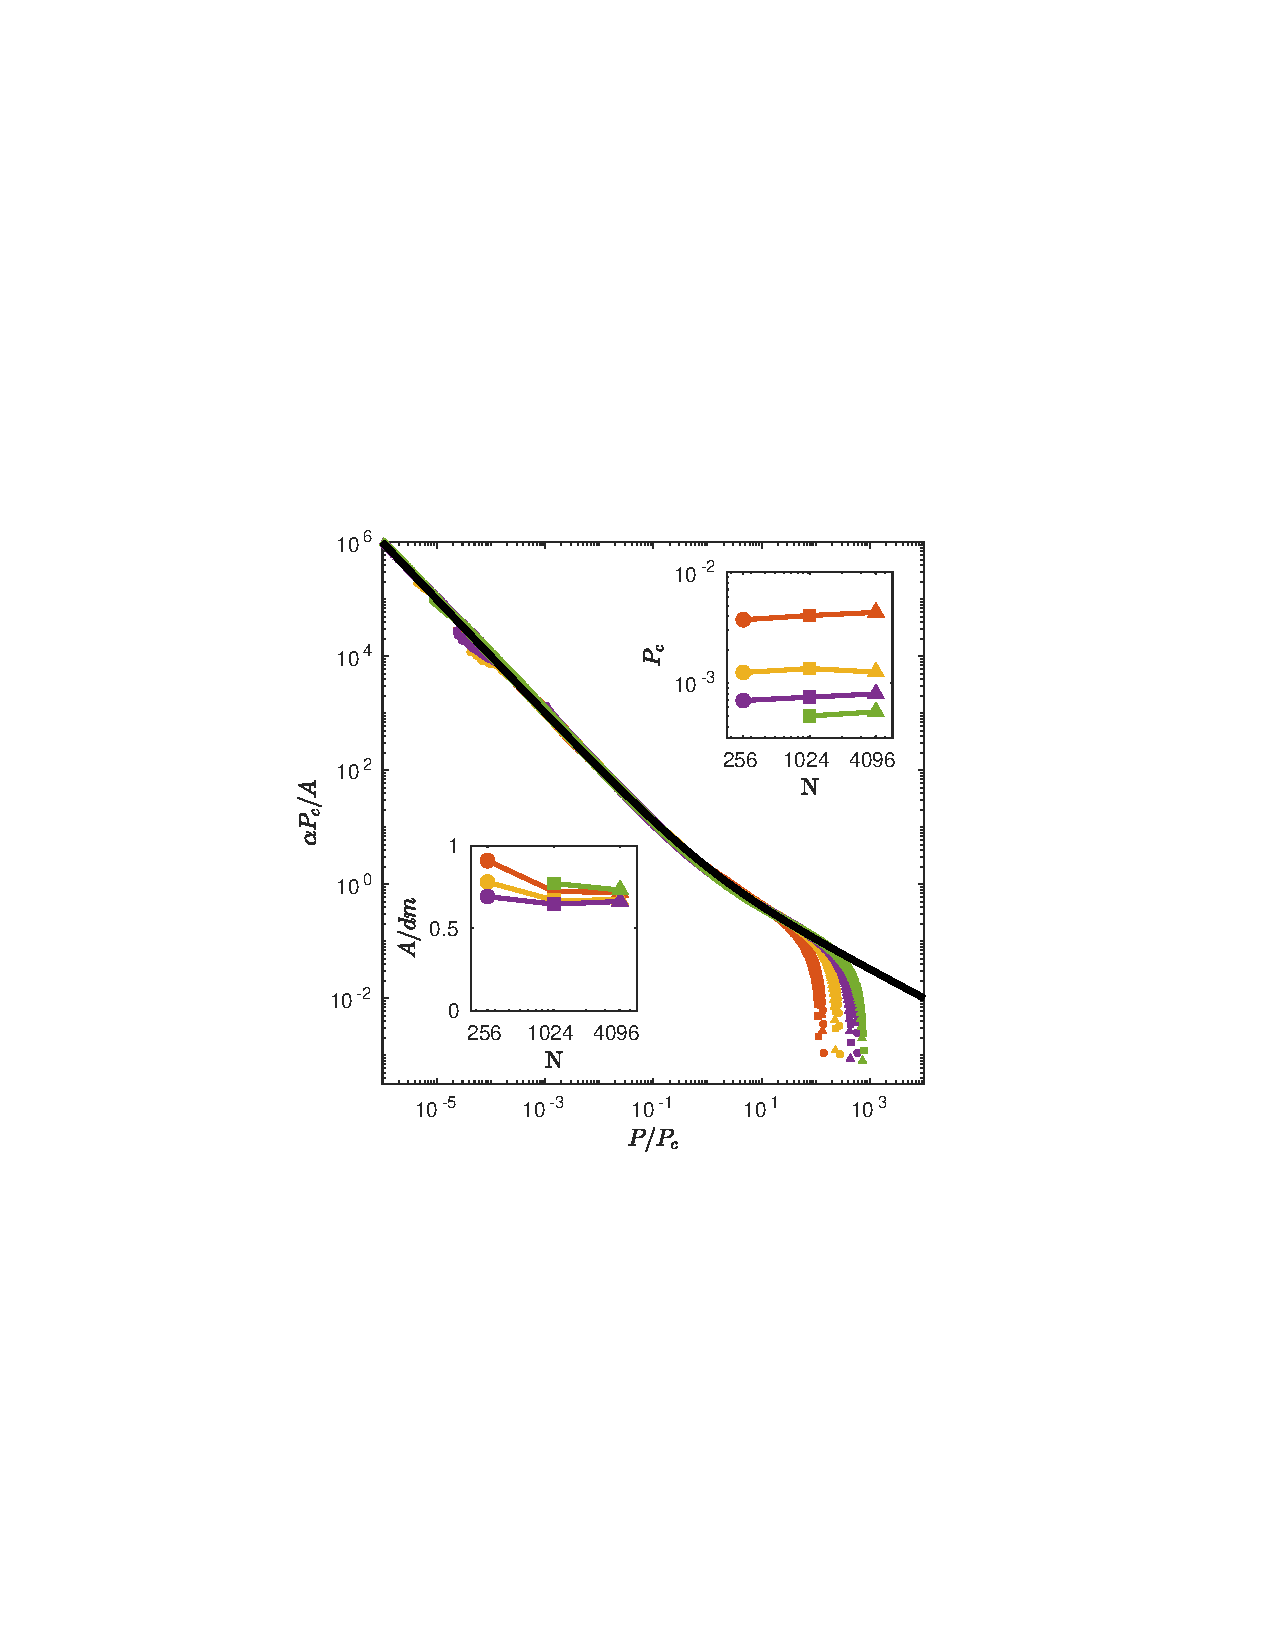
\includegraphics[width=\columnwidth, trim=143 240 165 253, clip]{forceVolumeEntropyPaper/angoricityInset.pdf}
\caption{Scaled angoricity, $\alpha P_c/A$, for all $N$ and $d$, collapses onto equation \ref{eqn:angoricity} (black line) when plotted against scaled pressure, $P/P_c$, until high pressure deviations caused by second nearest neighbor interactions. Inset top right, the crossover pressure $P_c$. Inset bottom left, $A/dm$ is approximately 0.7. Colors denote dimension from 2-5 and symbol denotes number of particles as in figure \ref{volumePlot}.
}
\label{angoricityPlot}
\end{figure}

\section{Discussion}
From Eq. (\ref{pc_equation}) and our measured values of $\gamma$ and $P_c$ we compute $h_f$, shown in the inset to Fig. \ref{lnhgPlot}. A complete expression for entropy can now be written as
%
\begin{align}
S &= \ln P + \Delta Z \ln\left(\frac{\gamma}{h_f}\right).
\end{align}
This can be recast into a natural form using \cref{eqn:excess,eqn:angoricityFittingForm} by expressing the ratio of $\gamma$ and $h_f$ as a critical number of excess contacts per particle, 
\begin{align}
\delta z_c &= 2B \sqrt{P_c}= \frac{2}{N\ln\left( \frac{\gamma}{h_f}\right)} \\
S &= \ln P + \frac{\delta z}{\delta z_c}. \label{eqn:finalEntropy}
\end{align}
%
Thus, the entropy is dependent on two intensive thermodynamic variables, $P$ and $\delta z$, and a constant $\delta z_c$ for each dimension. While $h_f$ is observed to decrease with $N$ and expected to vanish in the thermodynamic limit, we find $\delta z_c$ to be intensive with system size, as shown in Fig.~\ref{lnhgPlot}.

The first term in Eq. (\ref{eqn:finalEntropy}) describes the entropy increasing from the absolute pressure scale, whereas the second describes the entropy increasing from the number of contacts increasing. Sufficiently close to jamming the first term will dominate as there will be few changes in the contact network even as the pressure changes dramatically. Further from jamming the second term will dominate, reflecting the primacy of changes in the contact network.
Note that while this equation may be rewritten as a function of pressure using Eq. (\ref{eqn:excess}), for any particular finite packing the integer number of excess contacts is required to calculate the entropy precisely.


\section{Conclusion} We have demonstrated that the force network ensemble framework can be used to directly compute the multiplicity of the force configurations in packings close to the critical jamming point. We have presented an ansatz linking the volume of the force configurational space associated with a packing to the entropy of the packing.  This entropy can be expressed as a function of pressure and is independently confirmed by measurements of the angoricity over approximately seven orders of magnitude of pressure.  We have combined these two approaches of measuring entropy in order to extract the fundamental scales governing the discretization of phase space that allows for enumeration. We discover a crossover value for the excess contacts per particle, $\delta z_c$, below which the entropy is governed primarily by changes in pressure at fixed contact network and above which the entropy is governed primarily by the creation of new contact forces.

This work places angoricity on a firm footing as a thermodynamic quantity that controls the behavior of overjammed systems.  By tracing this entropy all the way down to an enumeration of states we discover that, perhaps unsurprisingly, Planck's constant does not set the fundamental scale of discretization $h_f$. In a purely classical model such as this, the discretization can only depend on the finite size effects of the system which are determined by $N$ and $d$. Thus, in the thermodynamic limit, while $h_f$ vanishes, the behavoir of the system is controlled by $\delta z_c$ and thus $P_c$ which do obtain fixed values. This full expression for entropy provides the first concrete linking of the microscopic force network ensemble to the thermodynamic description of granular materials and offers a complete description for the thermodynamics of the force networks in overjammed systems.

\section{Acknowledgments} We thank Bulbul Chakraborty, Karen Daniels, Sean Ridout, and Brian Tighe for useful discussions. This work benefited from access to the University of Oregon high performance computer, Talapas. This work was supported by National Science Foundation (NSF) Career Award DMR-1255370 and the Simons Foundation Grant No. 454939.

\begin{figure}[ht!]
\centering
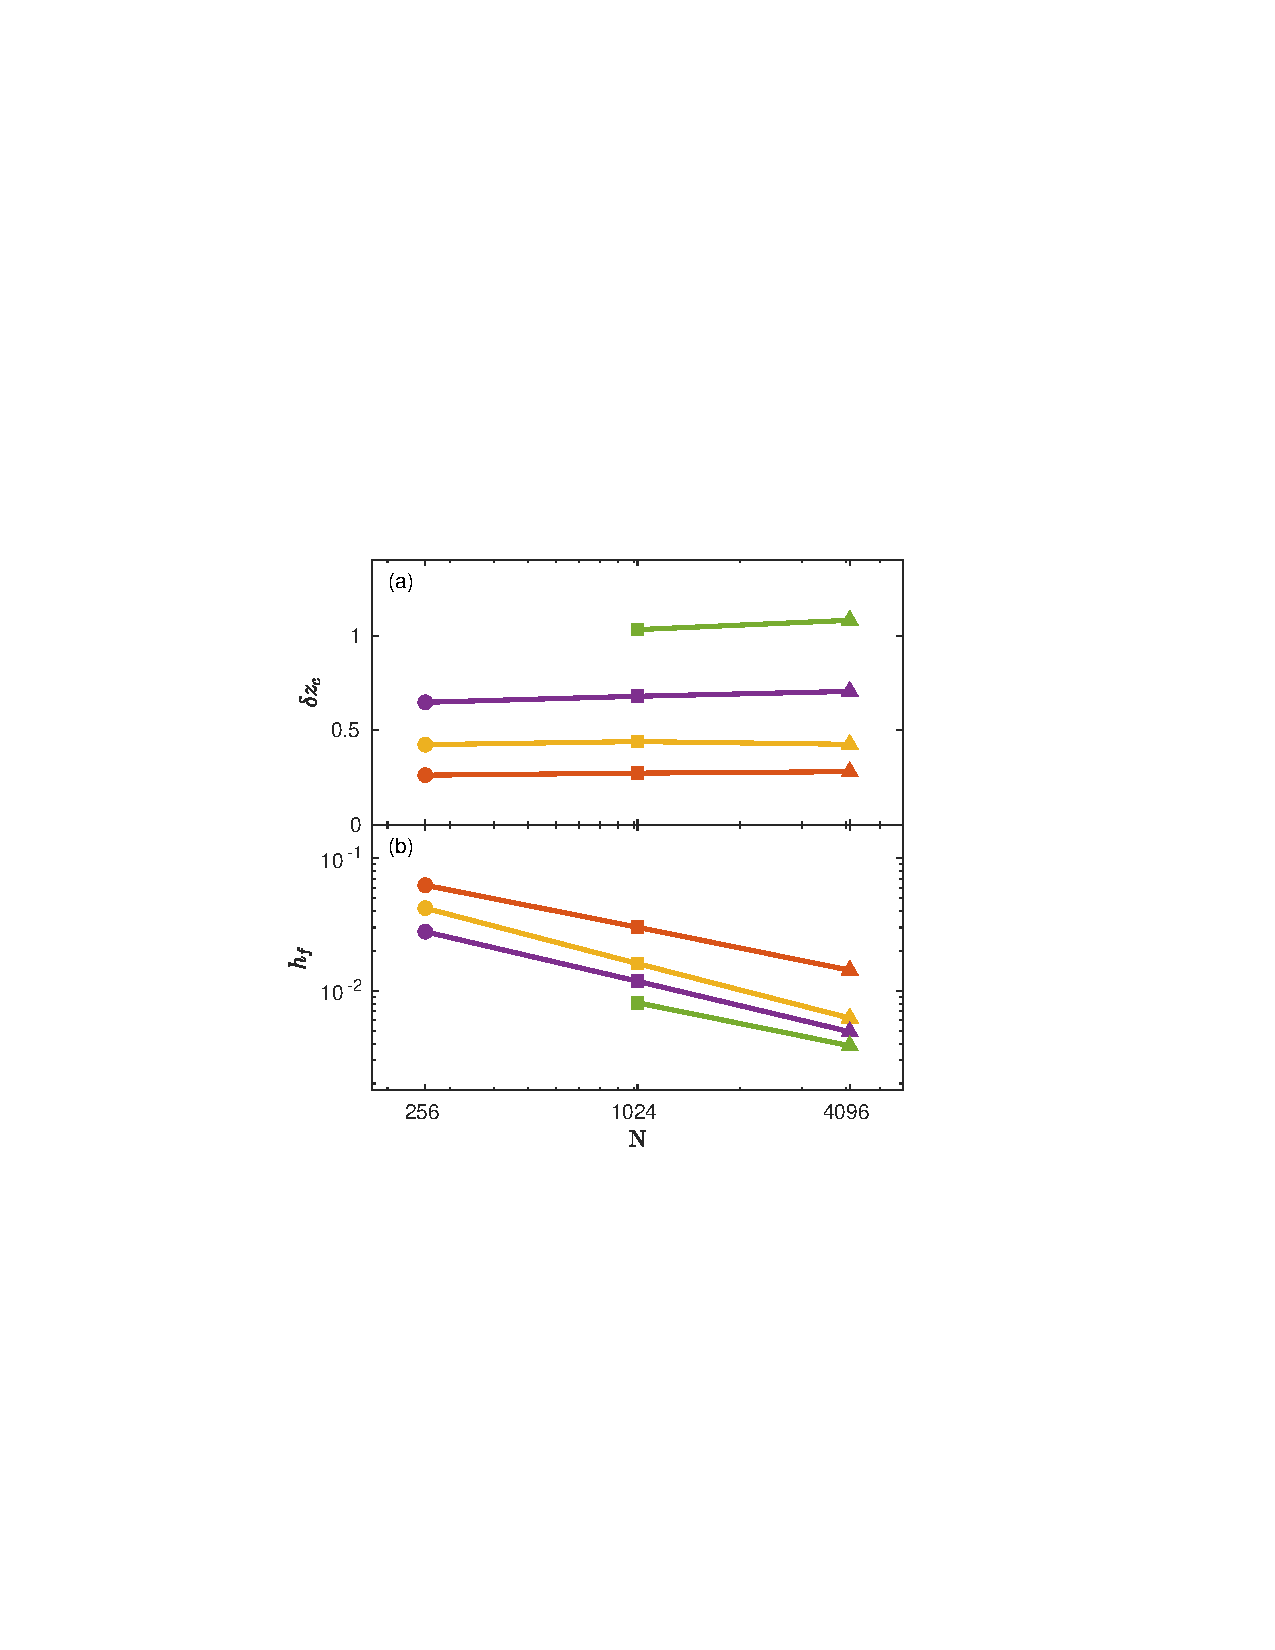
\includegraphics[width=\columnwidth, trim=138 254 176 268, clip]{forceVolumeEntropyPaper/lnhg.pdf}
\caption{Upper, scaling of $\delta z_c$ with $N$ and $d$. Lower, scaling of $h_f$, with $N$ and $d$, calculated from $P_c$ by inverting equation \ref{pc_equation}.  Colors denote dimension from 2-5 and symbol denotes number of particles as in figure \ref{volumePlot}. }
\label{lnhgPlot}
\end{figure}
%\bibliography{Angoricity}% Produces the bibliography via BibTeX.

%\end{document}
%
% ****** End of file aipsamp.tex ******



\chapter{Mean-Field Predictions of Scaling Prefactors Match Low-Dimensional Jammed Packings}
\author{James D. Sartor, Sean A. Ridout, Eric I. Corwin}
%\affiliation{$^*$Department of Physics and Materials Science Institute, University of Oregon, Eugene, Oregon 97403, USA \\ $^\dagger$Department of Physics and Astronomy University of Pennsylvania, Philadelphia, Pennsylvania 19104, USA}

\label{excessContactsScaling}

No known analytic framework precisely explains all the phenomena observed in jamming. The replica theory for glasses and jamming is a mean-field theory which attempts to do so by working in the limit of infinite dimensions, such that correlations between neighbors are negligible. As such, results from this mean-field theory are not guaranteed to be observed in finite dimensions. However, many results in mean field for jamming have been shown to be exact or nearly exact in low dimensions. This suggests that the infinite dimensional limit is not necessary to obtain these results. In this Letter, we perform precision measurements of jamming scaling relationships between pressure, excess packing fraction, and number of excess contacts from dimensions 2--10 in order to extract the prefactors to these scalings. While these prefactors should be highly sensitive to finite dimensional corrections, we find the mean-field predictions for these prefactors to be exact in low dimensions. Thus the mean-field approximation is not necessary for deriving these prefactors. We present an exact, first-principles derivation for one, leaving the other as an open question. Our results suggest that mean-field theories of critical phenomena may compute more for $d\geq d_u$ than has been previously appreciated.


 
\section{Introduction}
Granular materials exhibit universal properties regardless of the material properties of the individual grains \cite{liu_jamming_2010,charbonneau_universal_2012,charbonneau_glass_2017}.  The jamming transition is a critical point near which properties such as pressure, packing fraction, or number of excess contacts, among others, scale as power laws.  Scaling theory summarizes and condenses these power law relationships, but no first-principles theory of jammed systems at finite dimensions exists.  The replica mean-field theory of glasses and jamming has been shown to be exact in the infinite dimensional limit \cite{parisi_mean-field_2010,parisi_theory_2020}.  To do so it relies on the assumption that there are no correlations between neighbors, fundamentally at odds with low-dimensional systems. As such, mean-field predictions should not be expected to hold in low dimensional-jamming, and some results, most notably the packing fraction at jamming, deviate from the mean-field predictions \cite{charbonneau_universal_2012,parisi_robustness_2018}. However, despite the fact that low dimensional systems have highly correlated neighbors the scaling relations are precisely the same as those found in infinite dimensions \cite{ohern_jamming_2003, ohern_random_2002, goodrich_scaling_2016}. Many other results predicted by the mean field have also been observed in low dimensional jamming, suggesting that they may be provable without the mean field approximation \cite{charbonneau_universal_2012,charbonneau_universal_2016, berthier_perspective_2019,
charbonneau_glass_2017, dennis_jamming_2020,arceri_vibrational_2019}.

Here, we move one step further in the comparison between low-dimensional jamming and mean-field jamming by probing not only scaling relations but also prefactors between a handful of properties: pressure $P$, excess contacts $\delta z$, and excess packing fraction above jamming $\Delta \varphi$. We demonstrate the continued success of the mean field in describing low-dimensional systems by quantitatively verifying the mean-field predictions for these prefactors. Thus, the mean-field approximation is overzealous: one need not have vanishing correlations in order to obtain these results. In this spirit we provide a first-principles proof of the relation between pressure and excess packing fraction free of the mean-field assumptions.  These results call out for proofs for all of the other universal relations of the jamming transition.

\section{Background} Granular materials undergo a jamming transition at a critical packing fraction $\varphi_j$. The number of force bearing contacts between grains jumps abruptly from zero to the minimum number sufficient to support global rigidity and thus global pressure, $Z_c$. In a packing of $N$ frictionless, spherical particles in $d$ dimensions, $Z_c = Nd + 1 - d$~\cite{liu_jamming_2010, goodrich_finite-size_2012}.

We limit our study to spherical particles interacting through a harmonic contact potential given by 
%
 \begin{equation}
  U_{ij}= \eps \left(1-\frac{|\mathbf{r}_{ij}|}{\sigma_{ij}}\right)^2 \Theta\left(1-\frac{|\mathbf{r}_{ij}|}{\sigma_{ij}}\right),
 \end{equation}
%
where $\eps$ is the energy scale, $\mathbf{r_{ij}}$ is the contact vector between particles $i$ and $j$, $\sigma_{ij}$ is the sum of the radii of particles $i$ and $j$, and $\Theta$ is the Heaviside step function. Thus, the total energy $U= \frac{1}{2}\sum_{ij} U_{ij}$.
From this potential, the forces between particles can be calculated as
%
\begin{align}
 \mathbf{f}_{ij} &= \frac{2 \varepsilon}{\sigma_{ij}} \left(1-\frac{|\mathbf{r_{ij}}|}{\sigma_{ij}}\right) \Theta\left(1-\frac{|\mathbf{r_{ij}}|}{\sigma_{ij}}\right) \hat{r}_{ij}.
\end{align}
%
We compute a unit and dimension independent pressure using the microscopic formula \cite{ohern_jamming_2003,allen_computer_1989}
%
\begin{align}
 \label{eqn:stress_tensor_definition}
 P &\equiv -\frac{\bar{V}_p}{\varepsilon}\frac{d\utot}{dV}= \frac{\bar{V}_p}{\varepsilon Vd} \sum_{i,j} \mathbf{f}_{ij} \cdot \mathbf{r}_{ij}, 
 %\sum_{k} \mathbf{f}_\alpha^k \mathbf{r}_\beta^k
 \end{align}
 %
where $V$ is the volume of the system and $\bar{V}_p$ is the average particle volume. 


For soft spheres the packing fraction $\varphi$ can be increased, leading to new contacts and an increased pressure. We thus consider three natural quantities that measure distance from jamming:
\begin{itemize}
 \item excess packing fraction, $\Delta \varphi = \varphi - \varphi_j$
 \item excess contacts per particle, $\delta z=\left(Z-Z_c\right) / N$ where $Z$ is the number of contacts
 \item pressure $P$
\end{itemize}



The relationships between these quantities are predicted by mean-field theory as \cite{parisi_theory_2020}:
%
\begin{align}
P&=C_{p\varphi}\Delta \varphi \label{eqn:pvsphi} \\ 
\delta z&=C_{zp}P^{1/2} \label{eqn:evsp} 
\end{align}
%
with prefactors $C_{p\varphi}$ and $C_{zp}$ which are functions only of spatial dimension~\cite{ohern_jamming_2003}. These and other scaling relationships have been previously explained by approximate theories \cite{wyart_effects_2005, wyart_rigidity_2005,zaccone_approximate_2011,liarte_jamming_2019} and computationally confirmed in low-dimensional jamming \cite{ohern_jamming_2003, ohern_random_2002,liu_jamming_2010,goodrich_finite-size_2012}. They are summarized concisely by the scaling theory of the jamming transition~\cite{goodrich_scaling_2016}. The scaling exponents in $d \geq2$ match those in mean field, suggesting that the transition behaves like a critical point with upper critical dimension $d_u=2$.  Moreover, mean-field theory predictions of these prefactors can be derived as \cite{parisi_theory_2020,franz_universality_2017}:
\begin{align}
C_{p\varphi} &=   \frac{1}{d} \hat{C}_{p\varphi} \label{eqn:meanFieldPressurePhi}\\
C_{zp} &= \frac{d}{\sqrt{2^{d}}} \hat{C}_{zp} \label{eqn:meanFieldExcessPressure}
 \end{align}
where $\hat{C}_{p\varphi}$ and $\hat{C}_{zp}$ are finite constants in the $d\rightarrow\infty$ limit, which have not yet been explicitly calculated. Note that these relations are presented in a particular choice of units in the literature. We include details of the conversion to our dimensionless units in the Supplemental Material. \textit{A priori}, it is not expected that these predictions will apply in low dimensions, in which the mean-field assumption is not warranted. Even above upper critical dimensions, mean-field theories are not generally expected to correctly compute prefactors, or even the purportedly universal amplitude ratios. Beyond scaling exponents, to our knowledge, the critical cluster shape in percolation and related phenomena \cite{aronovitz_universal_1987,privman_universal_1991} and the Binder cumulant in the Ising model \cite{brizin_finite_1985, parisi_scaling_1996, blote_universality_1997} are the only quantities which are known to be equal to their mean-field values above the upper critical dimension. Even though these prefactors for jamming scaling relationships have been measured and reported \cite{ohern_jamming_2003,sartor_direct_2020}, because they are not expected to be equal to their mean-field values they have not received substantial theoretical attention. An approximate calculation of the related prefactor between the shear modulus and number of excess contacts has been performed in three dimensions \cite{zaccone_approximate_2011}.

%
\begin{figure}[h!]
%carefully picked
%adding some whitespace at the top
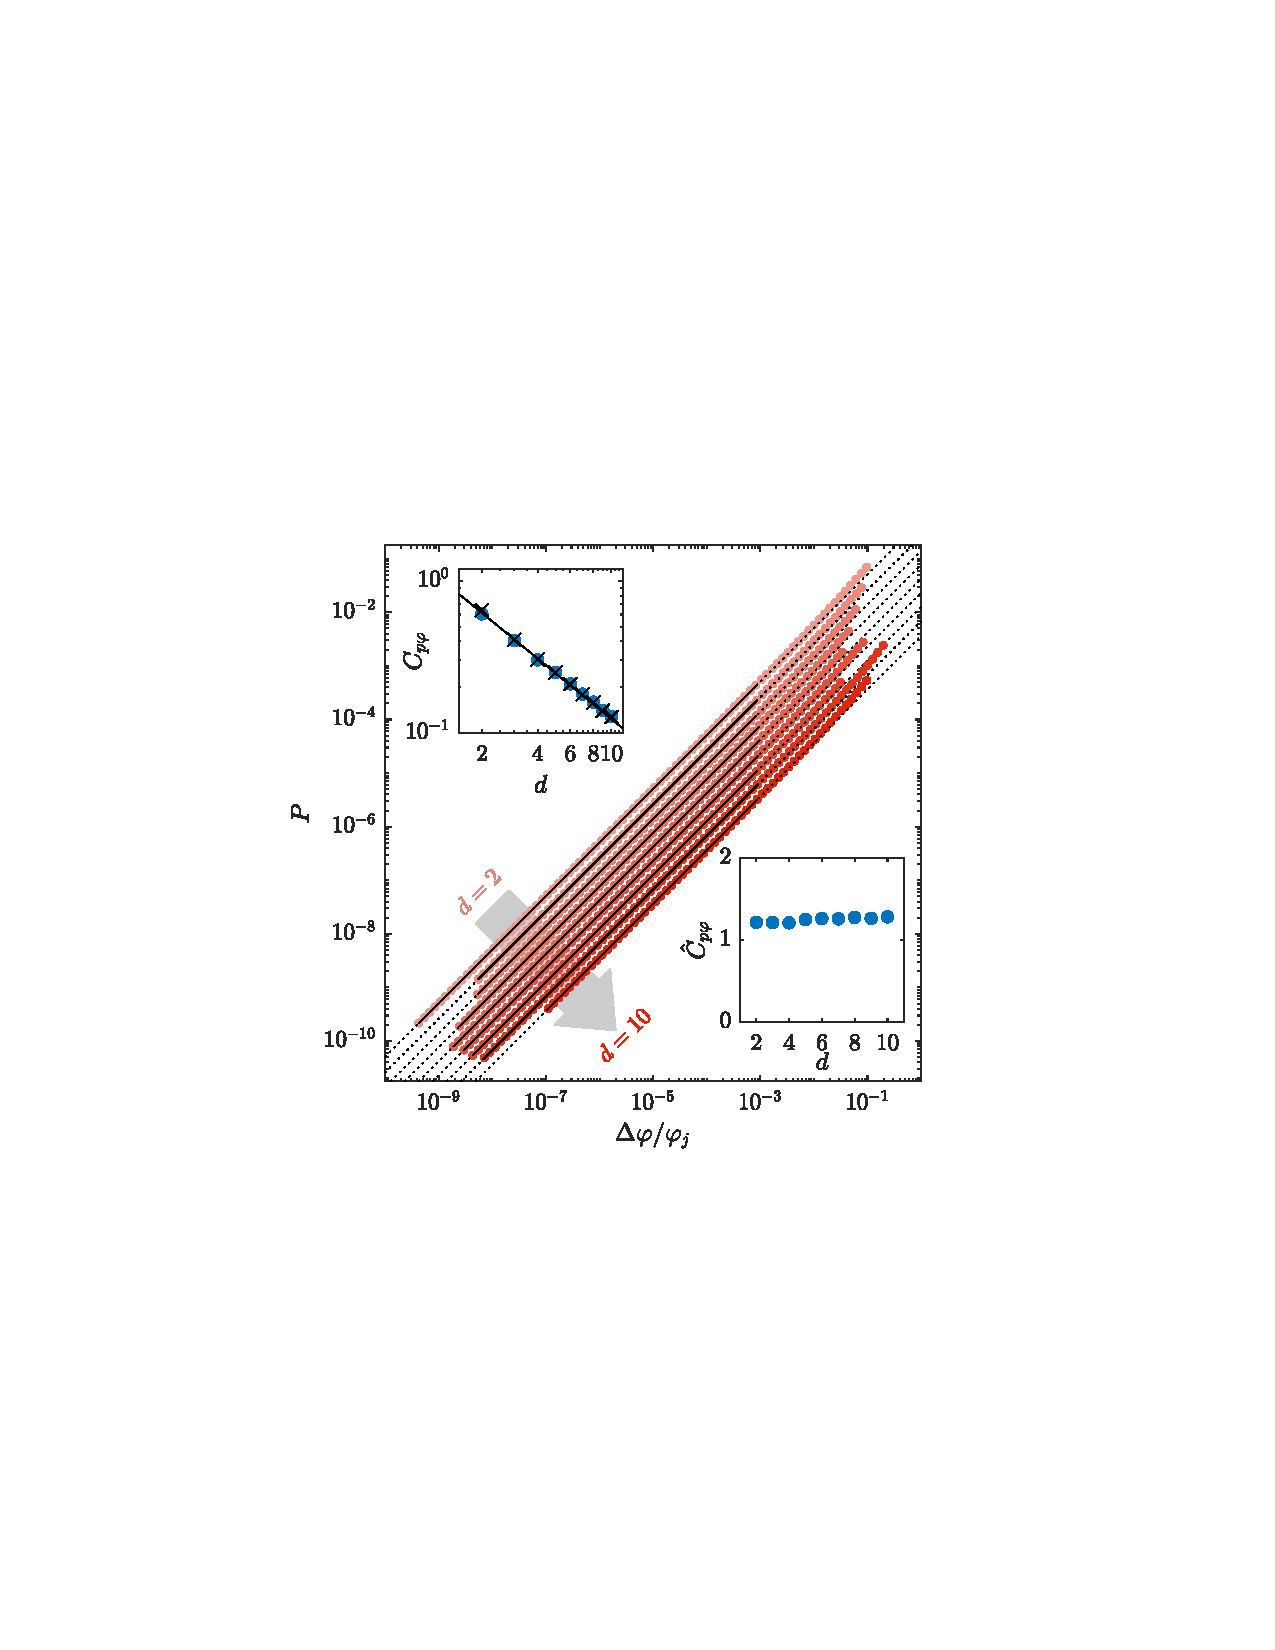
\includegraphics[width=\columnwidth, trim=140 241 169 241, clip]{excessContactsScaling/pvsphiSub.pdf}
%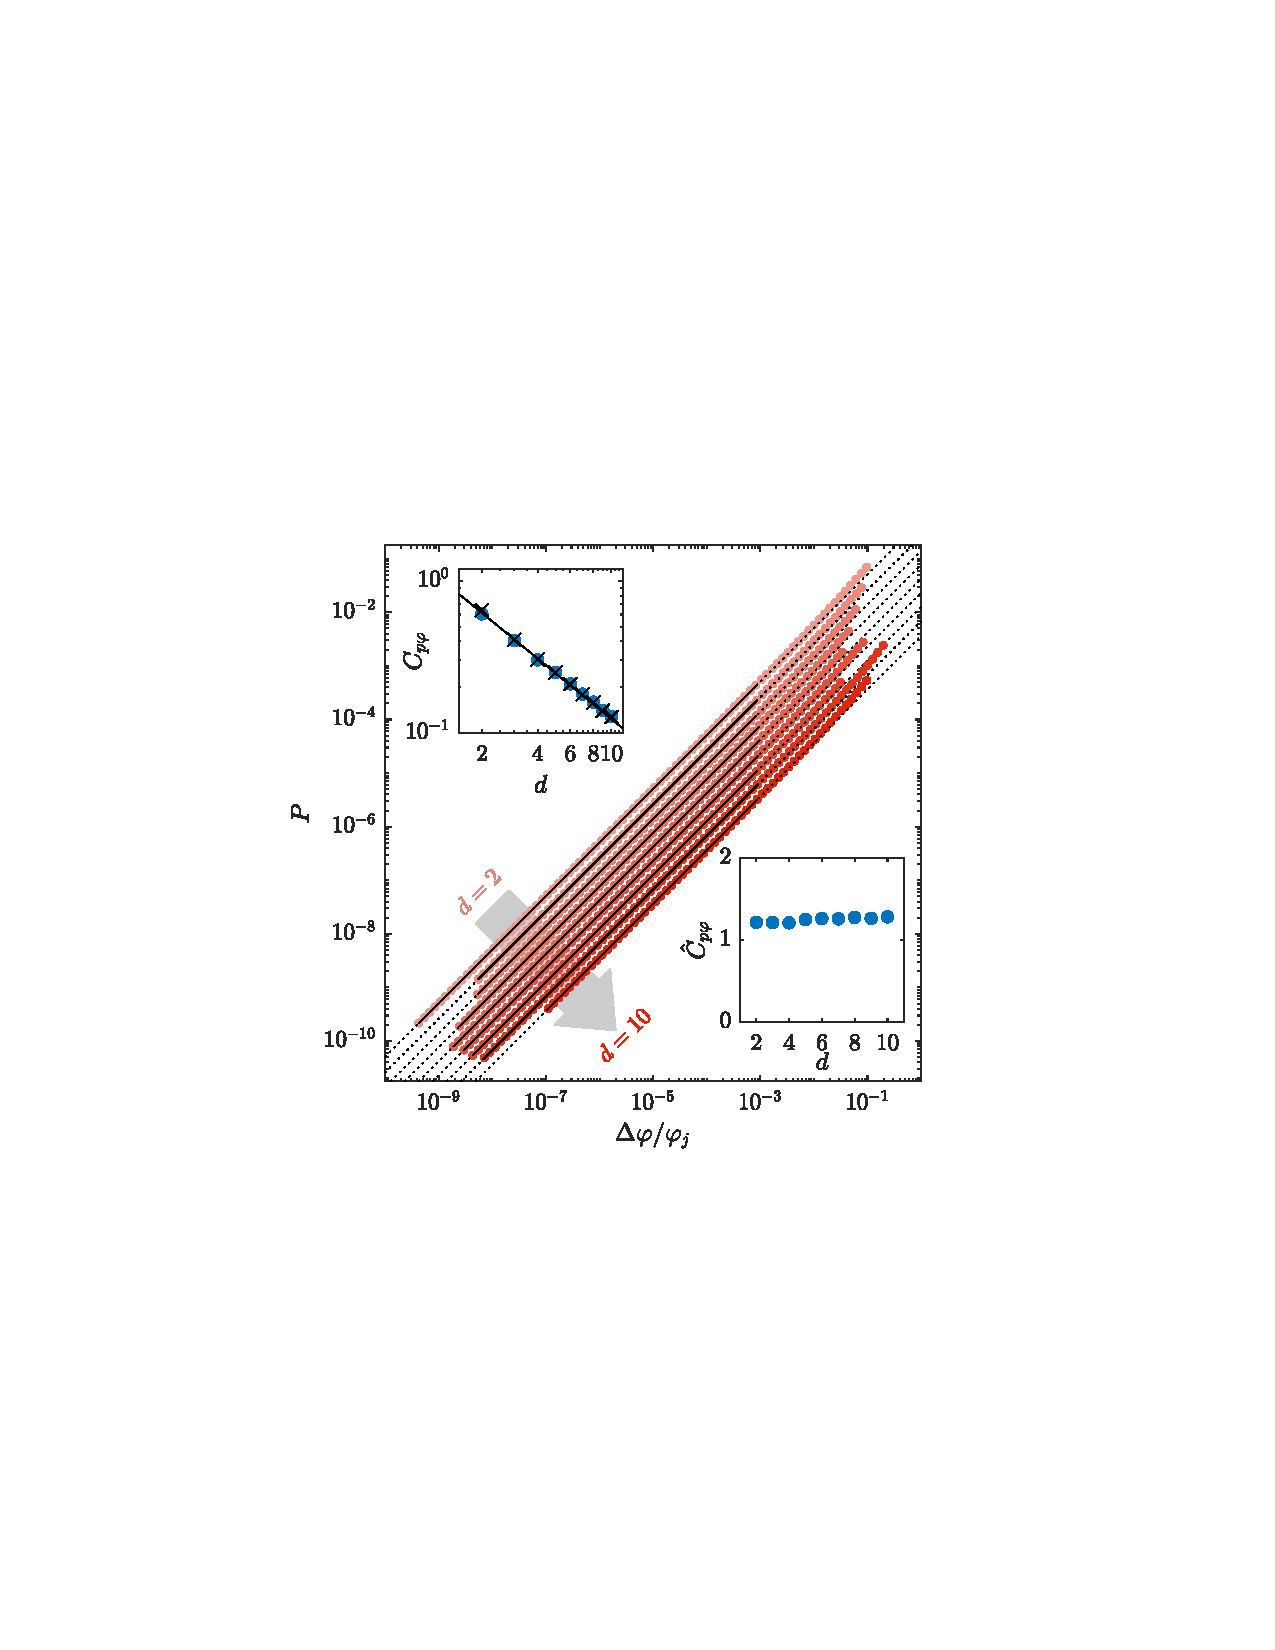
\includegraphics[width=\columnwidth, trim=140 241 169 261, clip]{excessContactsScaling/pvsphiSub.pdf}
\caption{Measured pressure scales linearly with scaled excess packing fraction for systems from $d=2$ to $d=10$. Measured values for $\varphi_j$ in our protocol are included in the Supplemental Material. Black lines show fits for $C_{p\varphi}$ using Eq. \ref{eqn:pvsphi}. We exclude from the fit data with $\Delta\varphi/\varphi_j>10^{-3}$, to avoid the effect of larger overlaps causing deviations from this power law. Dotted lines show the extension of fits beyond fitted range. Upper inset shows the measured values of $C_{p\varphi}$ (blue circles) to scale in agreement with the mean-field prediction Eq. \ref{eqn:meanFieldPressurePhi}, shown as a fit to a black line with $\hat{C}_{p\varphi} \approx 1.23$. Moreover, they are in precise agreement with predicted values from Eq. \ref{eqn:seanPrediction} (marked with black $\cross$'s). Lower inset shows measured values of $\hat{C}_{p\varphi}$ calculated from the measured values of $C_{p\varphi}$ and eqn \ref{eqn:meanFieldPressurePhi}. While each prefactor is measured from a single system, the prefactors for a second, identically constructed dataset were calculated to be well within the bounds of the marker size.}
%https://www.latimes.com/socal/burbank-leader/opinion/tn-blr-me-aword-20181005-story.html
\label{plot:pvsphi}
\end{figure}
%
%
\begin{figure}[h!]
%carefully picked
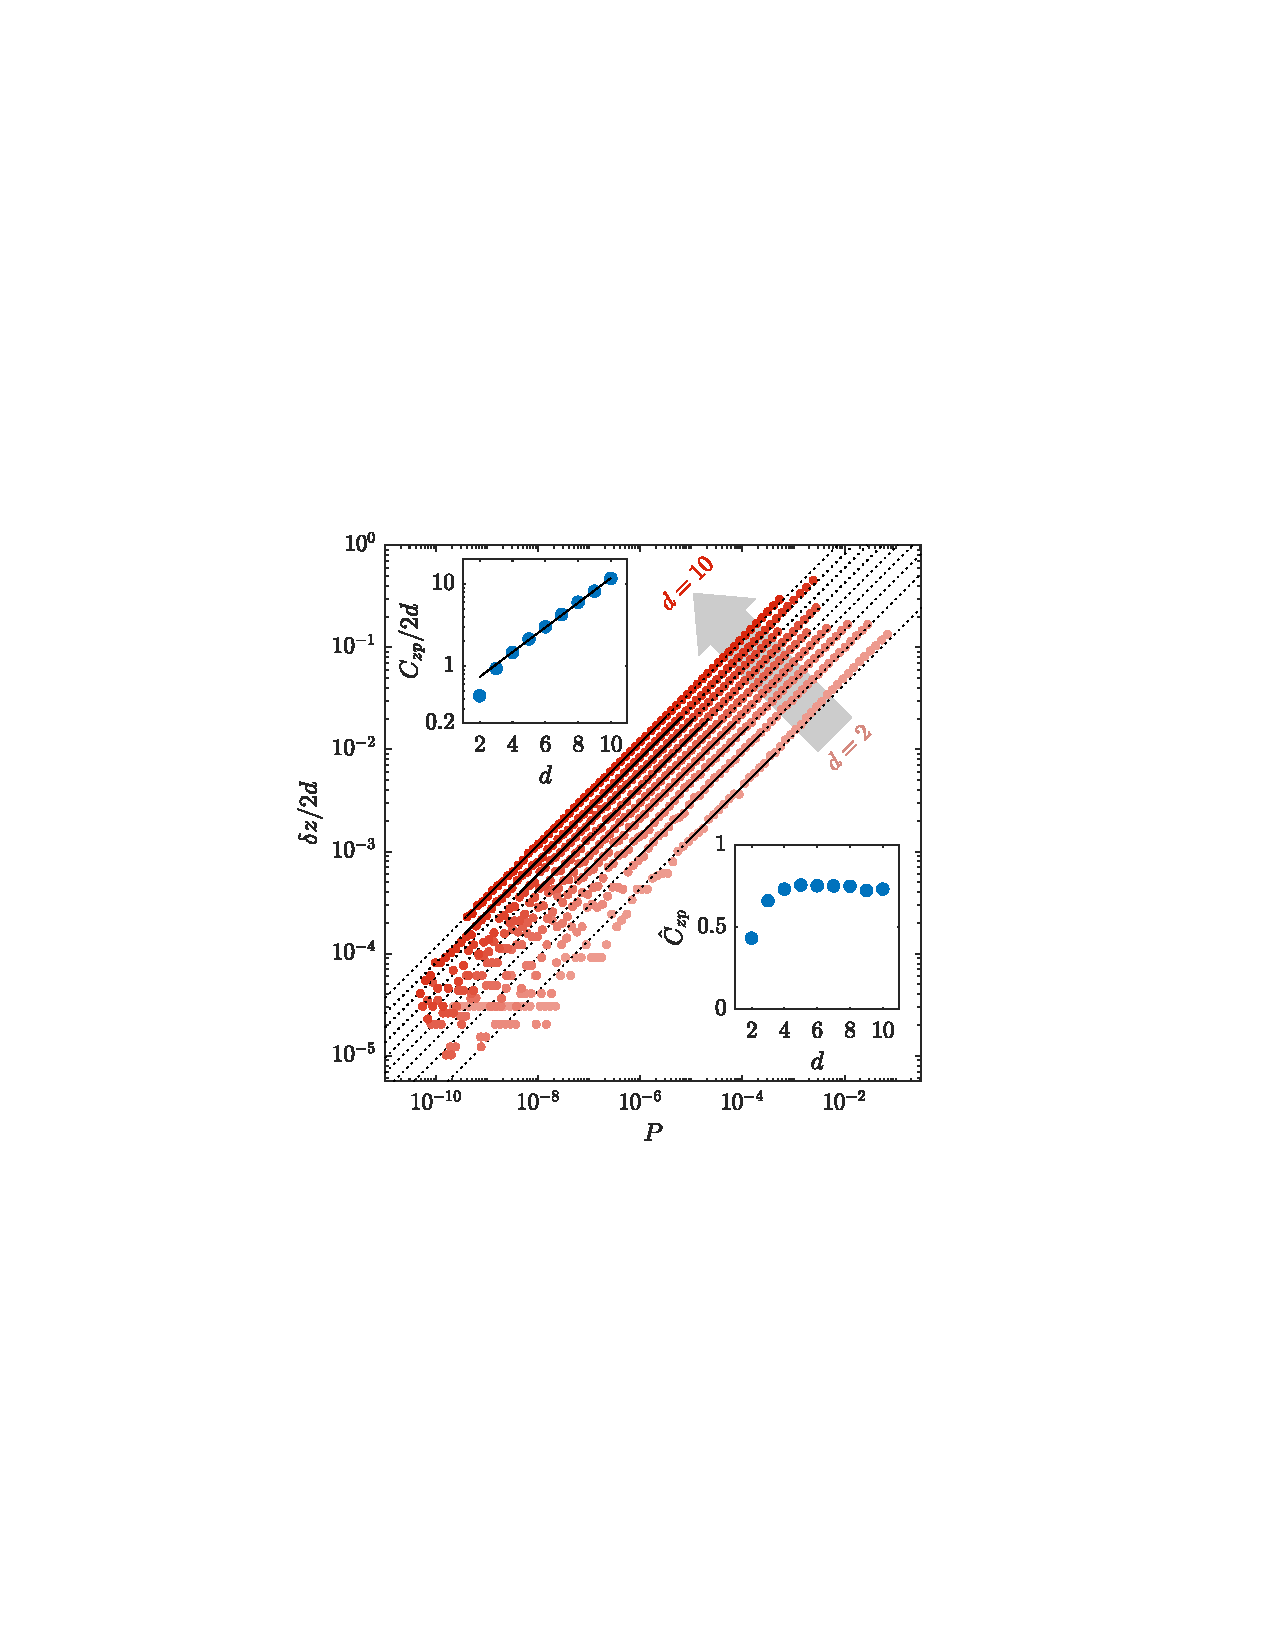
\includegraphics[width=\columnwidth, trim=143 244 169 235, clip]{excessContactsScaling/evspSub.pdf}
%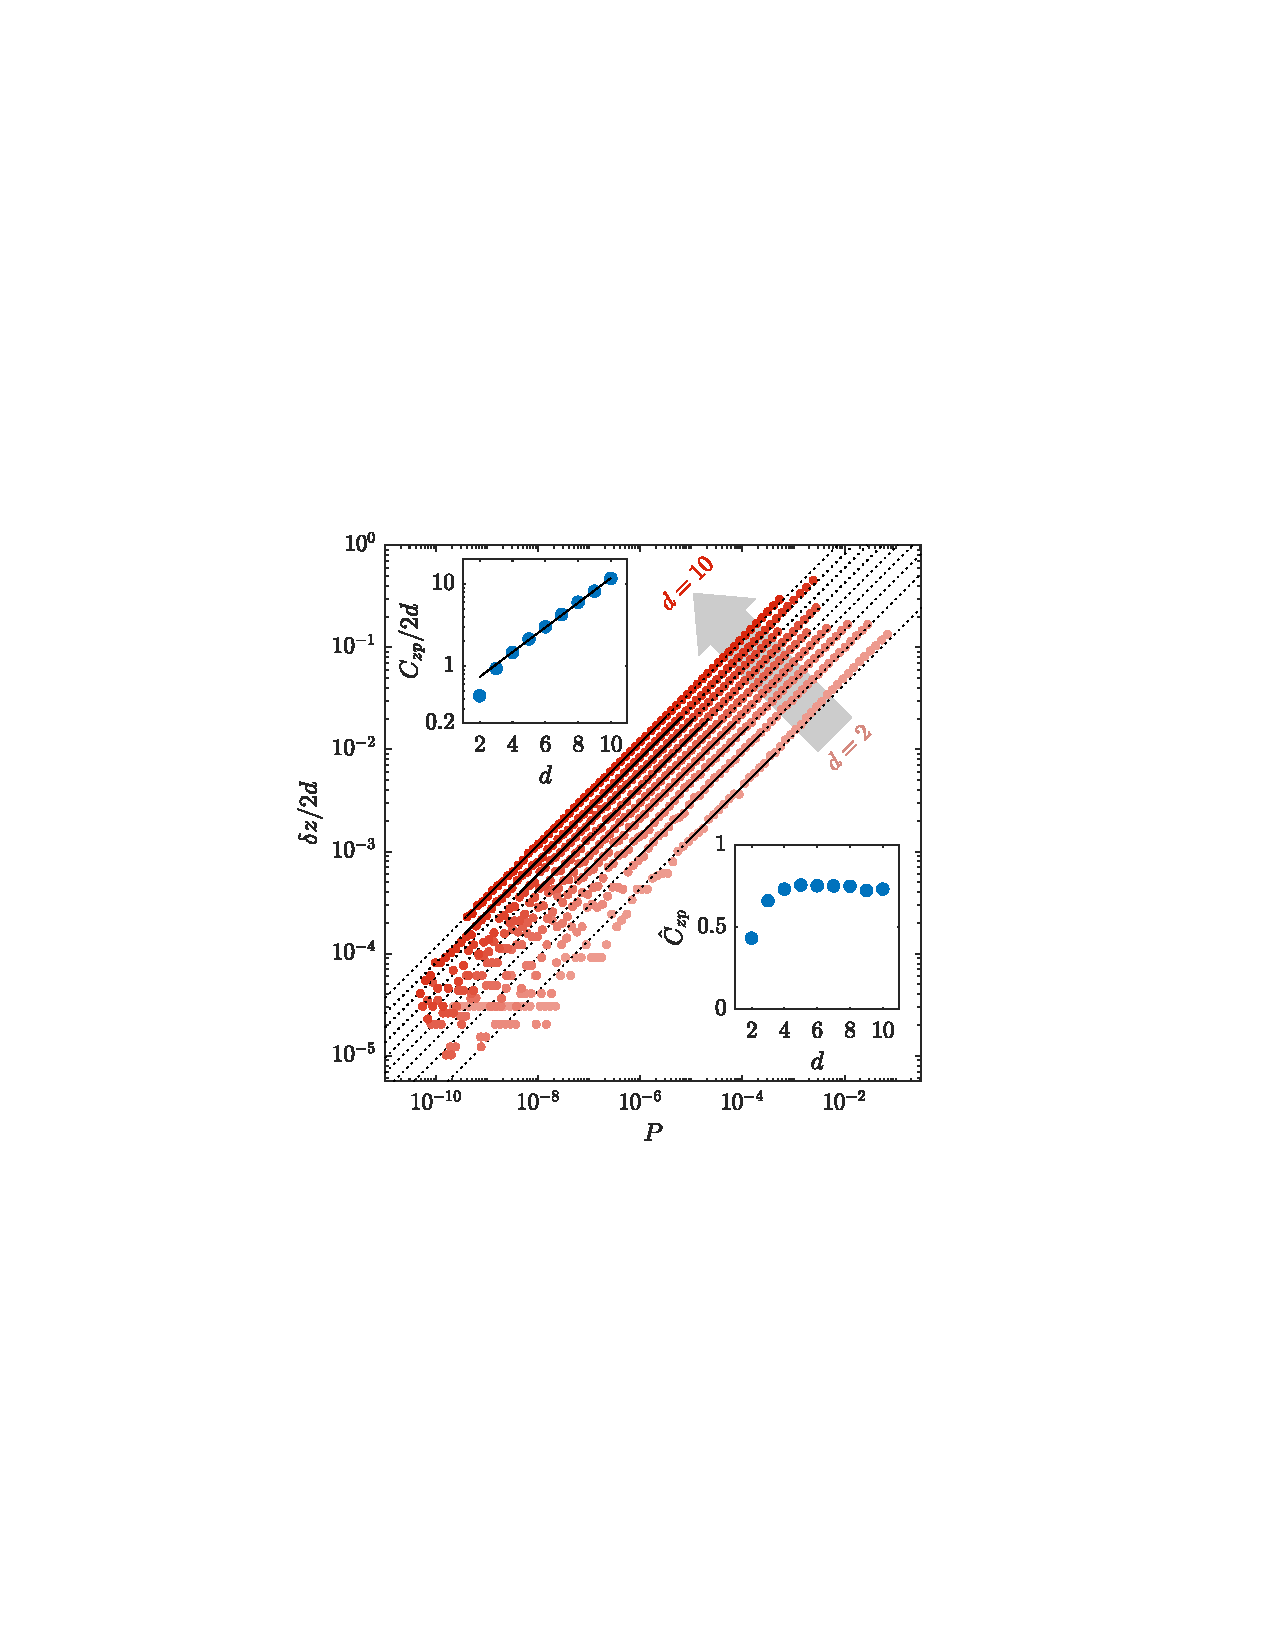
\includegraphics[width=\columnwidth, trim=143 244 169 255, clip]{excessContactsScaling/evspSub.pdf}
\caption{  Measured excess contacts scales with the square root of pressure for systems from $d=2$ to $d=10$. Black lines show fits for $C_{zp}$ using Eq. \ref{eqn:evsp}. For our fits, we ignore high pressure data as in Fig. \ref{plot:pvsphi}, and additionally exclude data with less than 40 excess contacts to avoid fitting to small number fluctuations. Dotted lines show the extension of our fits beyond fitted range. Lower inset shows the measured values of $C_{zp}$ (blue circles), which scale in agreement with the mean-field prediction Eq. \ref{eqn:meanFieldExcessPressure}, shown as a fit to a black line and with $\hat{C}_{zp} \approx 0.74$.  Upper inset shows measured values of $\hat{C}_{zp}$ calculated from the measured values of $C_{zp}$ and Eq. \ref{eqn:meanFieldExcessPressure}. While each prefactor is measured from a single system, the prefactors for a second, identically constructed dataset were calculated to be well within the bounds of the marker size.}
\label{plot:evsp}
\end{figure}
%
\section{Computational methods}
We use pyCudaPacking~\cite{charbonneau_universal_2012}, a GPU-based simulation engine, to generate energy minimized soft (or penetrable) sphere packings. We do so for number of particles $N=8192-32768$ and dimension $d=2-10$. Our results suggest that $N=8192$ is large enough to avoid finite size effects in $d<9$, which we have verified in $d=8$ by comparing our packing at $N=8192$ with one at $N=16384$, finding no deviation. For $d=9$ and $d=10$ we use system sizes of $16384$ and $32768$, respectively. The particles are monodisperse, except in two dimensions in which we use equal numbers of bidisperse particles with a size ratio of 1:1.4 to prevent crystallization.
 
 The packings are subject to periodic boundary conditions. We minimize the packings using the FIRE minimization algorithm \cite{bitzek_structural_2006} using quad precision floating point numbers in order to achieve resolution on the contact network near the jamming point.
 
 Using the same methods as described in Ref. \cite{charbonneau_jamming_2015}, we start with randomly distributed initial positions, and apply a search algorithm to create systems approximately logarithmically spaced in $\Delta\varphi$. At each step we use the known power law relationship between energy and $\Delta\varphi$ to calculate an estimate of $\varphi_j$. We use this estimate to approximate $\Delta\varphi$ and determine the next value of $\varphi$ in an effort to logarithmically space $\Delta\varphi$ values. We then adjust the packing fraction to this value of $\varphi$ by uniformly scaling particle radii and minimizing the system. We continue this process until the system is nearly critically jammed, i.e. has exactly one state of self stress. We then use the known power law relationship between pressure and $\Delta\varphi$ to fit the dataset and precisely calculate $\varphi_j$ (with error less than the smallest value of $\Delta\varphi$) from which we calculate $\Delta\varphi$ at each value of $\varphi$.
 
 \section{Results}
 Figure \ref{plot:pvsphi} shows the measured linear scaling of pressure with packing fraction separately for each dimension. We fit the data to Eq. \ref{eqn:pvsphi} to find $C_{p\varphi}$, considering only data close to jamming to avoid fitting to high pressure deviations from the scaling power law. The measured values of $C_{p\varphi}$ are shown in the inset to confirm the $1/d$ dimensional scaling predicted by mean-field theory in Eq. \ref{eqn:meanFieldPressurePhi}. A fit to this scaling provides a value of $\hat{C}_{p\varphi}$ of 1.23.

Figure \ref{plot:evsp} shows the measured square root scaling of excess contacts with pressure separately for each dimension. We fit the data to Eq. \ref{eqn:evsp} to find $C_{zp}$, the values of which are shown in the inset. Beginning around three dimensions, the values of $C_{zp}$ confirm the dimensional scaling predicted by mean-field theory in Eq. \ref{eqn:meanFieldExcessPressure}, and a fit to this scaling provides a value of $\hat{C}_{zp}$ of 0.74.

The values of both $C_{p\varphi}$ and $C_{zp}$ are roughly consistent with values measured in previous studies \cite{ohern_jamming_2003, sartor_direct_2020}. It has been recently suggested that the prestress, i.e., the normalized ratio of the first and second derivatives of the potential as defined in Ref.~\cite{shimada_low-frequency_2019}, is a better candidate to dedimensionalize the relationship between pressure and excess contacts. However, we find a substantially better collapse of our expected form of pressure than with prestress. For more details on prestress, see the attached Supplemental Material.

\section{Discussion}
The close agreement of our data with the mean-field predictions in low dimensions suggests that the mean-field assumption is not essential to derive these scaling and prefactor relations. In the spirit of discovering proofs for these relations free of the mean-field assumption, we expand on an earlier calculation of the bulk modulus scaling \cite{wyart_rigidity_2005} to show that such a calculation can also explain the scaling of $C_{p \varphi}$ with spatial dimension and the precise value of $\hat{C}_{p \varphi}$.


From taking a derivative of Eq. \ref{eqn:pvsphi}, we see immediately that $C_{p\varphi}$ may be expressed in terms of the bulk modulus, $K\equiv V\frac{d^2U}{dV^2}$, at jamming:
%
\begin{equation} 
C_{p \varphi} = \frac{\mpv V}{ \varphi \varepsilon}  \frac{d^2 \utot}{dV^2} = \frac{V}{N \varepsilon } K \label{eqn:CisK}.
\end{equation}
%
We note that this approximation slightly overestimates $C_{p\varphi}$: the apparently linear average stress-strain curves of jammed packings are actually the average of many piecewise linear curves with discontinuous drops in stress, thus the average slope is slightly less than the instantaneous slope \cite{fan_particle_2017}.

At the unjamming point, the linear response of the system is that of a network of unstretched springs. Thus, at lowest order in pressure the bulk modulus is that of an unstressed spring network,  which may be calculated in terms of the ``states of self stress,'' vectors of possible spring tensions, $s\in \mathbb{R}^{Z}$, which do not produce any net force on a particle \cite{pellegrino_structural_1993, wyart_rigidity_2005, lubensky_phonons_2015}. Here we explain how to carry out this calculation for a monodisperse system in the unjamming limit; a correction for polydispersity is handled in the Supplemental Material.

We begin by defining the set of ``affine bond extensions,'' a vector $E \in \mathbb{R}^{Z}$ giving the amount by which each bond vector would increase under a unit volumetric expansion of the system. In linear elasticity, this simply induces an expansion of each length by $1/d$, so,

\begin{equation}
E_{\ell} = \frac{1}{d} r_{\ell}\label{eqn:affine},
\end{equation}

where we emphasize that $\ell$ indexes the contacts in the system rather than the particles; $r_{\ell}$ is the distance between a particular pair of particles.

In the case that all springs have the same spring constant $k$ (e.g., monodisperse packings), the bulk modulus may be written as the projection of these affine moduli onto the states of self stress \cite{pellegrino_structural_1993, wyart_rigidity_2005, lubensky_phonons_2015}. At jamming, there is only one state of self stress, and so the bulk modulus may be computed exactly using the projection onto only this one state of self stress \cite{wyart_rigidity_2005},
%
%\begin{align}
%    C_{p\varphi} &= \frac{\color{NavyBlue}{P}}{\color{ForestGreen}{\Delta \varphi}} \\
%    &= \color{ForestGreen} {\left( \frac{d\varphi}{dV}\right)^{-1}}\color{NavyBlue} \frac{dP}{dV}  \\ 
%    &= \color{ForestGreen}\frac{V}{N} \color{NavyBlue}{\frac{K}{\varepsilon}}
%\end{align}
%
%
\begin{align}
    K&= \frac{k}{V}  \left(\sum_{\ell = 1}^{Z} s_{1,\ell} E_{\ell}  \right)^2\label{eqn:sssproj} \\
    &=\frac{2 N \eps}{ d V} \frac{\langle  f \rangle^2}{\langle f^2 \rangle}
\end{align}
%
In the near jamming limit, this one special state of self stress exists all the way down to the jamming point and can be expressed in terms of the vector of physical force magnitudes, $f$. For the packing to be in equilibrium, this set of contact forces must produce no net force on every particle, and thus by definition the vector $f$ is always a state of self stress. The projection defined above requires states of self stress to be normalized, and so the state of self stress may be expressed as:

\begin{equation}
s_{1,\ell}= \frac{1}{\sqrt{\sum_l f_l }} f_{\ell} = \frac{1}{\sqrt{Z \langle f^2 \rangle}} f_{\ell}. \label{eqn:sss}
\end{equation}

Furthermore at lowest order in $P$ we have $r = \sigma$, and we assume $Z \approx d N$. Thus, Eq.  \ref{eqn:sssproj} reduces to 

\begin{align}
    K&= \frac{N k \sigma^2}{ d V} \frac{\langle  f \rangle^2}{\langle f^2 \rangle} = \frac{2 N \eps}{ d V} \frac{\langle  f \rangle^2}{\langle f^2 \rangle}
\end{align}


and thus via Eq. \ref{eqn:CisK}
 
\begin{equation}
    C_{p\varphi} = \frac{2}{d} \frac{\langle f \rangle^2}{\langle f^2 \rangle},
\end{equation}
for monodisperse spheres. The full calculation in the Supplemental Material shows that in the polydisperse case this becomes
\begin{equation}
    C_{p\varphi} = \frac{2}{d} \frac{\langle \sigma f \rangle^2}{\langle \sigma^2 f^2 \rangle}.\label{eqn:seanPrediction}
\end{equation}

We find that the distribution of contact forces does not depend strongly on dimension, which we demonstrate and discuss in the Supplementary Material, including Refs. \cite{charbonneau_jamming_2015,mueth_force_1998}. We thus predict the scaling of $C_{p \varphi}$ to agree with the asymptotic mean-field scaling. Because this proof does not invoke the mean-field assumption, we expect this scaling to be correct in all dimensions. Moreover, we are able to calculate each value of $C_{p\varphi}$ by measuring the ratio of force distribution moments. These values are calculated as in Eq. \ref{eqn:seanPrediction}, and are shown in Fig. \ref{plot:pvsphi} to precisely predict the values of $C_{p\varphi}$. 

\section{Conclusion}
The mean-field theory of jamming predicts both the scaling exponents and the dimensional scaling of their prefactors. While the exponents have been previously verified, we have demonstrated that even some prefactors are well predicted in low dimensions by mean-field theory. Although these prefactors should be considered especially sensitive to finite dimensional corrections, we find the mean field prediction to be exact in low dimensions. Is this a generic phenomenon, or are the quantities we have chosen to study in this work somehow specially unaffected by finite dimensional correlations? Experience with critical phenomena suggests that although certain ratios of these prefactors (i.e. amplitude ratios) may be universal, the prefactors themselves should be both nonuniversal and challenging to compute, which has led to them being neglected. Our results demonstrate however that these prefactors may be computed exactly. These results call out for other theories of jamming and the glass transition which reproduce the mean-field results without such assumptions, or perhaps for a deeper understanding of why certain mean-field computations may be exact in finite dimensions. Additionally, our results suggest that in traditional critical phenomena mean-field theory may compute more for $d\geq d_u$ than has been previously appreciated.

%%

\section{Acknowledgments}
We thank Francesco Zamponi for generous assistance in interpreting the mean-field results. We also thank Andrea Liu, Jim Sethna, Cam Dennis, and Aileen Carroll-Godfrey for valuable discussion and feedback. This work benefited from access to the University of Oregon high performance computer, Talapas. This work was supported by National Science Foundation (NSF) Career Grant No. DMR-1255370 and the Simons Foundation No. 454939 (J.D.S. and E.I.C.) and by an NSERC PGS-D fellowship and Simons Foundation No. 454945 to Andrea J. Liu. (S.A.R.). 

%\bibliography{scaling}% Produces the bibliography via BibTeX.


%\end{document}
%
% ****** End of file aipsamp.tex ******



\section{Supplementary Material of ``Mean-field predictions of scaling prefactors match low-dimensional jammed packings''}
\author{James D Sartor, Sean A. Ridout, Eric I. Corwin}
%\affiliation{$^*$Department of Physics and Materials Science Institute, University of Oregon, Eugene, Oregon 97403, USA \\ $^\dagger$Department of Physics and Astronomy University of Pennsylvania, Philadelphia, PA 19104, USA}
%\maketitle

\label{excessContactsScalingSupplement}
%\onecolumn

\subsection{Measured values of $\varphi_j$}
In Table \ref{table:phij} we show our measued values of $\varphi_j$. these values are used in calculating $\Delta \varphi$.

\begin{table}[ht]
\caption{Measured values of $\varphi_j$ in dimensions 2-10.
\label{table:phij}}
\begin{tabular}{ |c|c|c|c|c|c|c|c|c|c| } 
 \hline
 d & 2 & 3 & 4 & 5 & 6 & 7 & 8 & 9 & 10 \\ 
 \hline
 $\varphi_j$ & 0.85 & 0.65 & 0.46 & 0.31 & 0.20 & 0.13 & 0.078 & 0.049 & 0.029\\ 
 \hline
\end{tabular}
\end{table}

\subsection{Mean Field Prediction of Pressure vs Packing Fraction}

Mean field theory predicts that pressure scales with packing fraction as follows \cite{parisi_theory_2020}:
\begin{align}
 \hat{P} &= \hat{C}(\hat{\varphi} - \hat{\varphi}_j) \label{sup_eqn:pvsphi}
 \end{align}
 where $\hat{C}_{p\varphi}$ is a constant, and the hats over $P$ and $\Delta \varphi$ signify that the quantities are scaled such to be fixed in the infinite dimensional limit, as follows:
 \begin{align}
\hat{P} &= \frac{P^*}{\rho d} \label{sup_eqn:phat} \\
\hat{\varphi} &= \frac{2^d}{d} \varphi %= \frac{\bar{V_p}}{d} \rho
 \end{align}
where $\rho$ is the number density, $\frac{N}{V}$, and $P^*$ is the pressure which is calculated with assumed unit particle diameter. This relates to our pressure, $P$, as follows:
\begin{align}
 P & = \frac{\varphi}{\rho} \frac{1}{d^2} P^* \label{sup_eqn:pstar} , 
\end{align}
where the factor of $\frac{\varphi}{\rho}$ unwraps their assumption of unit particle diameter, and the factor of $\frac{1}{d^2}$ comes from their potential, which explicitly contains a dimensional term:
\begin{align}
 U^*(r) &= \frac{\epsilon d^2}{2} \left(\frac{r}{\ell}-1\right)^2 \Theta\left(\ell-r\right).
\end{align}
We can thus rewrite equation \ref{sup_eqn:phat} in terms of our pressure $P$:
\begin{align}
 \hat{P} &= \frac{d}{\varphi}P,
\end{align}
 and therefore equation \ref{sup_eqn:pvsphi}:
 \begin{align}
  \frac{d}{\varphi}P &=\hat{C}\frac{2^d}{d}( \varphi - \varphi_j) \\
  P &= \frac{\varphi}{d} \hat{C} \frac{2^d}{d} \Delta \varphi \\
  P &= \frac{1}{d}\hat{C}\hat{\varphi}_j( \Delta \varphi) \\
   P &= \frac{1}{d}\hat{C}_{p\varphi}( \Delta \varphi). \label{sup_eqn:finalpvsphi}
\end{align}
%
Where, noting that $\hat{\varphi}_j$ and $\hat{C}$ are constants in the infinite dimensional limit, we combine them as $\hat{C}_{p\varphi}$. Thus mean field predicts a simple $1/d$ scaling of the prefactor between pressure and excess packing fraction.


\subsection{Mean Field Prediction of Pressure vs Number Of Excess Contacts}

The number of contacts, $z$, is predicted by mean field theory to have the form \cite{parisi_theory_2020}:
%
\begin{align}
\frac{z}{2d} &=1 + \hat{C}_{z\varphi}\sqrt{\hat{\varphi}-\hat{\varphi_j}} \\
\frac{z}{2d} &=1 + \hat{C}_{z\varphi}\sqrt{\frac{2^d}{d}}\sqrt{\varphi-\varphi_j} \label{eqn:meanFieldExcessPhi}
\end{align}
%
for some constant $\hat{C}_{z\varphi}$. 

The number of excess contacts, $\delta z$, therefore is predicted to scale as follows:
\begin{align}
\frac{\delta z}{2d} &= \hat{C}_{z\varphi}\sqrt{\frac{2^d}{d}}\sqrt{\varphi - \varphi_j} \\ % the 1 goes away cuz it's dz
\delta z &= 2d\hat{C}_{z\varphi}\sqrt{\frac{2^d}{d}}\sqrt{\varphi - \varphi_j} \label{supeqn:finalphivsz}.
\end{align}


\subsection{Mean Field Prediction of Packing Fraction vs Number of Excess Contacts}

By combining equations \ref{sup_eqn:finalpvsphi} 
and \ref{supeqn:finalphivsz},
we can also predict the relation between $\delta z$ and $P$:
%
\begin{align}
 \delta z &= 2d\hat{C}_{z\varphi}\sqrt{\frac{2^d}{d}} \sqrt{\frac{d}{\hat{C}_{p\varphi}}P} \\
 &= 2d\hat{C}_{z\varphi}\sqrt{\frac{2^d}{\hat{C}_{p\varphi}}} \sqrt{P} \\
\end{align}
%
where we define $\hat{C}_{zp}=\frac{2\hat{C}_{z\varphi}}{\sqrt{\hat{C}_{p\varphi}}}$.

\begin{figure}[th!]
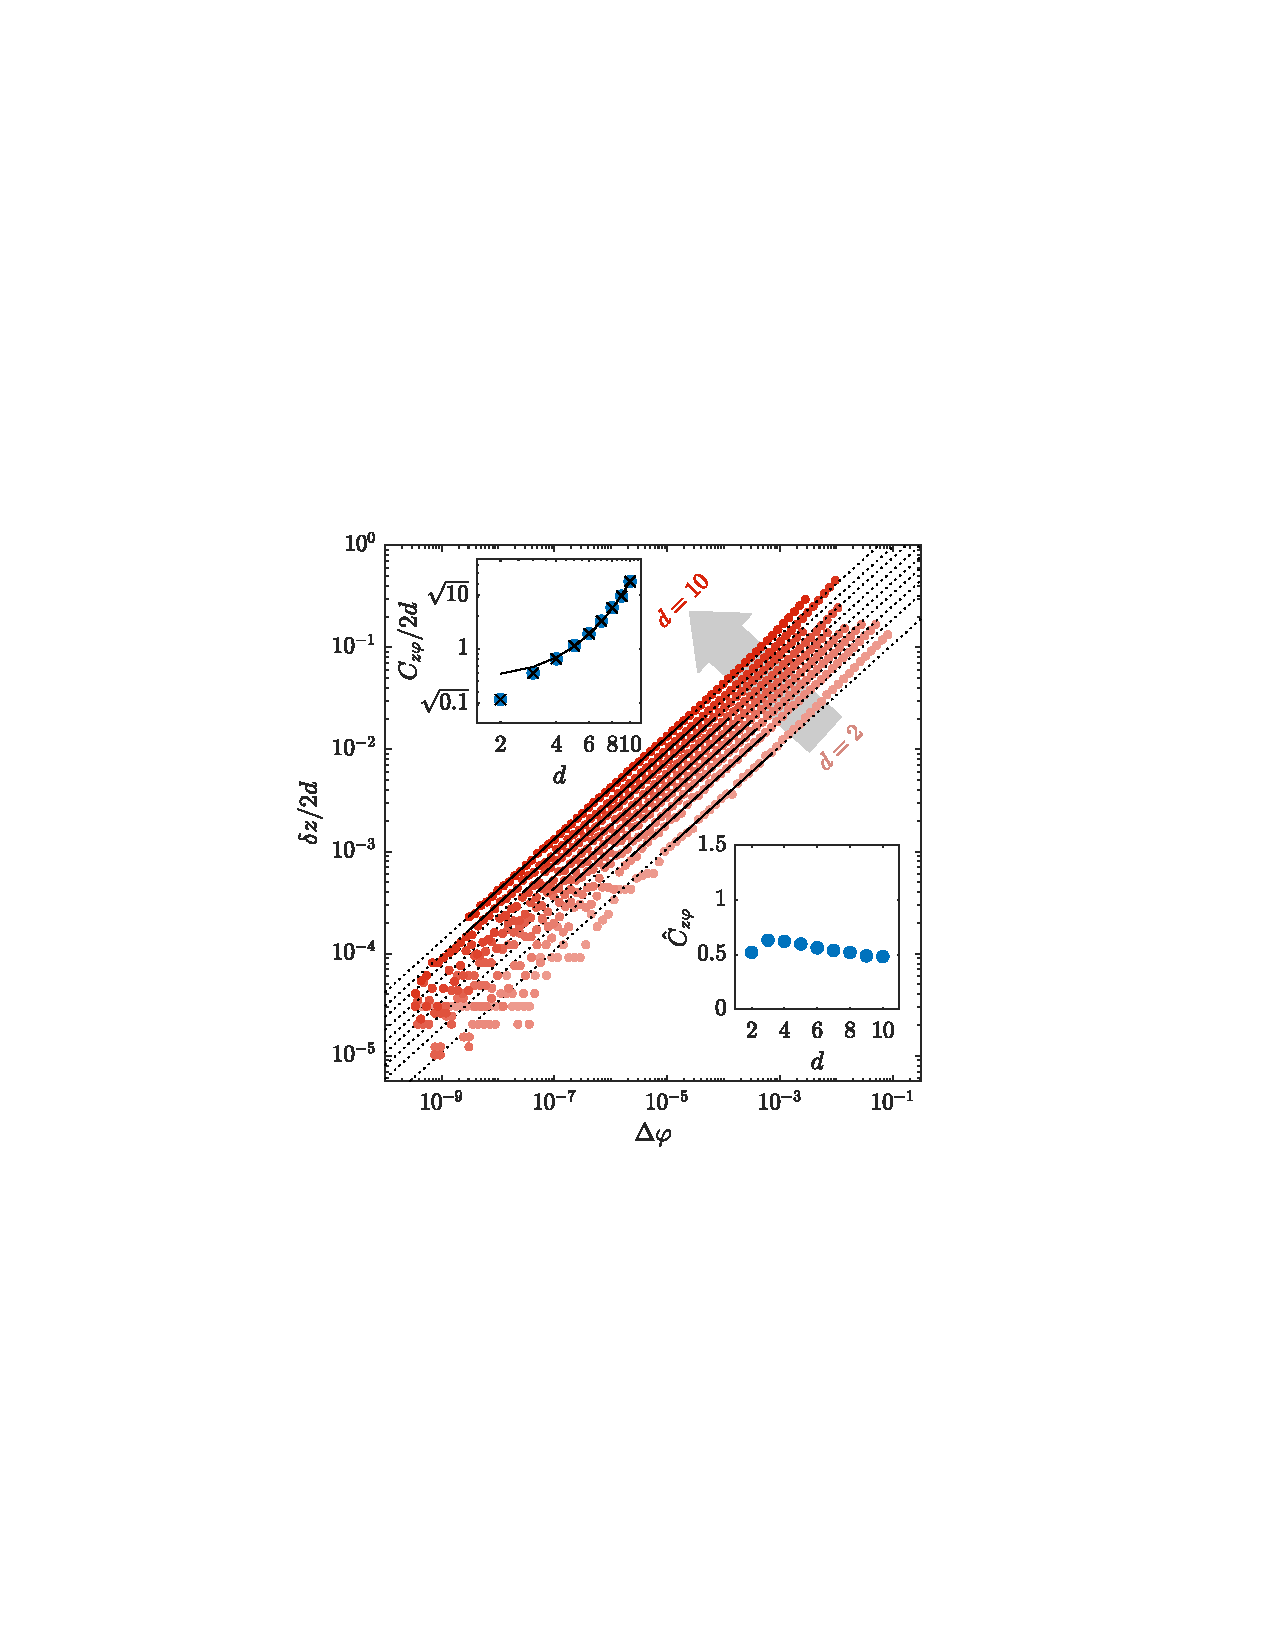
\includegraphics[width=300px, trim=143 240 168 250, clip]{excessContactsScaling/evsphi.pdf}

\caption{Measured excess contacts scales with the square root of excess packing fraction for systems from $d=2$ to $d=10$ (red circles). Black lines show the fits for $C_{zp}$ using eqn \ref{eqn:evsphi}. For our fits, we ignore data at high pressure and low contact number as in figure \ref{plot:evsp}.
Dotted lines show the extension of our fits beyond the fitted range. Inset shows the measured values of $C_{z\varphi}$ (blue circles), which scale in agreement with the mean field prediction eqn \ref{supeqn:finalphivsz} using measured values of with $\hat{C}_{z\varphi} \approx 0.83$. Additionally, to note consistency we show that our measured values of $C_{z\varphi}$ agree well with values calculated from our measurements of $C_{p\varphi}$ and $C_{zp}$ using eqn \ref{eqn:consistency} (black x's).}

\label{plot:evsphi}
\end{figure}
%
\subsection{Excess Contacts vs Excess Packing Fraction Prefactor Scaling}

From eqns \ref{eqn:pvsphi} and \ref{eqn:evsp} 
we can simply relate $\delta z$ and $\varphi$ as follows:
%
\begin{equation}
\delta z=C_{z\varphi}\left(\Delta\varphi\right)^{1/2} \label{eqn:evsphi}
\end{equation}
%
where clearly, 
\begin{align}
C_{z\varphi}=C_{zp}\sqrt{C_{p\varphi}}. \label{eqn:consistency}
\end{align}

In figure \ref{plot:evsphi}, we show this scaling seperately for each dimension. We fit each line to eqn \ref{eqn:evsphi} to find the values of the prefactor $C_{z\varphi}$ in each dimension, the values of which are shown in the inset. These values agree well with both the mean field prediction above $3D$, shown as a black line, and our calculated value from $C_{zp}$ and $C_{p\varphi}$, shown as black x's in figures \ref{plot:pvsphi} 
and \ref{plot:evsp}.

%
\subsection{Dimensional Dependence of Force Moment Ratios}
In figure \ref{plot:mfr} we show that the ratio of force moments does not depend strongly on dimension. This empirical fact may seem at odds with previous reports of how the low-force part of the distribution differs from its mean-field form in low dimensions \cite{charbonneau_jamming_2015,mueth_force_1998}. The low-force part of the distribution has $P(f) \propto f^\theta$, where $\theta\approx 0.17$ in $d=2$ smoothly rises to a $d=\infty$ value of $\theta \approx 0.42$. The high-force behaviour decays like an exponential or a stretched exponential; thus, we have computed the theoretical value of this moment ratio for distributions of the form $P(f) \sim f^\theta e^{-f /f_0}$ and $P(f) \sim f^\theta e^{-f^2 /f_0^2}$, as shown in figure \ref{plot:theory_mfr}. We find that neither of these assumed distributions quantitatively predicts the measured moment ratio for the known values of $\theta$, but they do show that the known variation in $\theta$ should not make us expect a large variation in this moment ratio.



\begin{figure}[h!]
%    \caption{Dimensional dependence of force moment ratios}
%  \label{plot:test}
%  \begin{subfigure}[t]{0.47\columnwidth}
  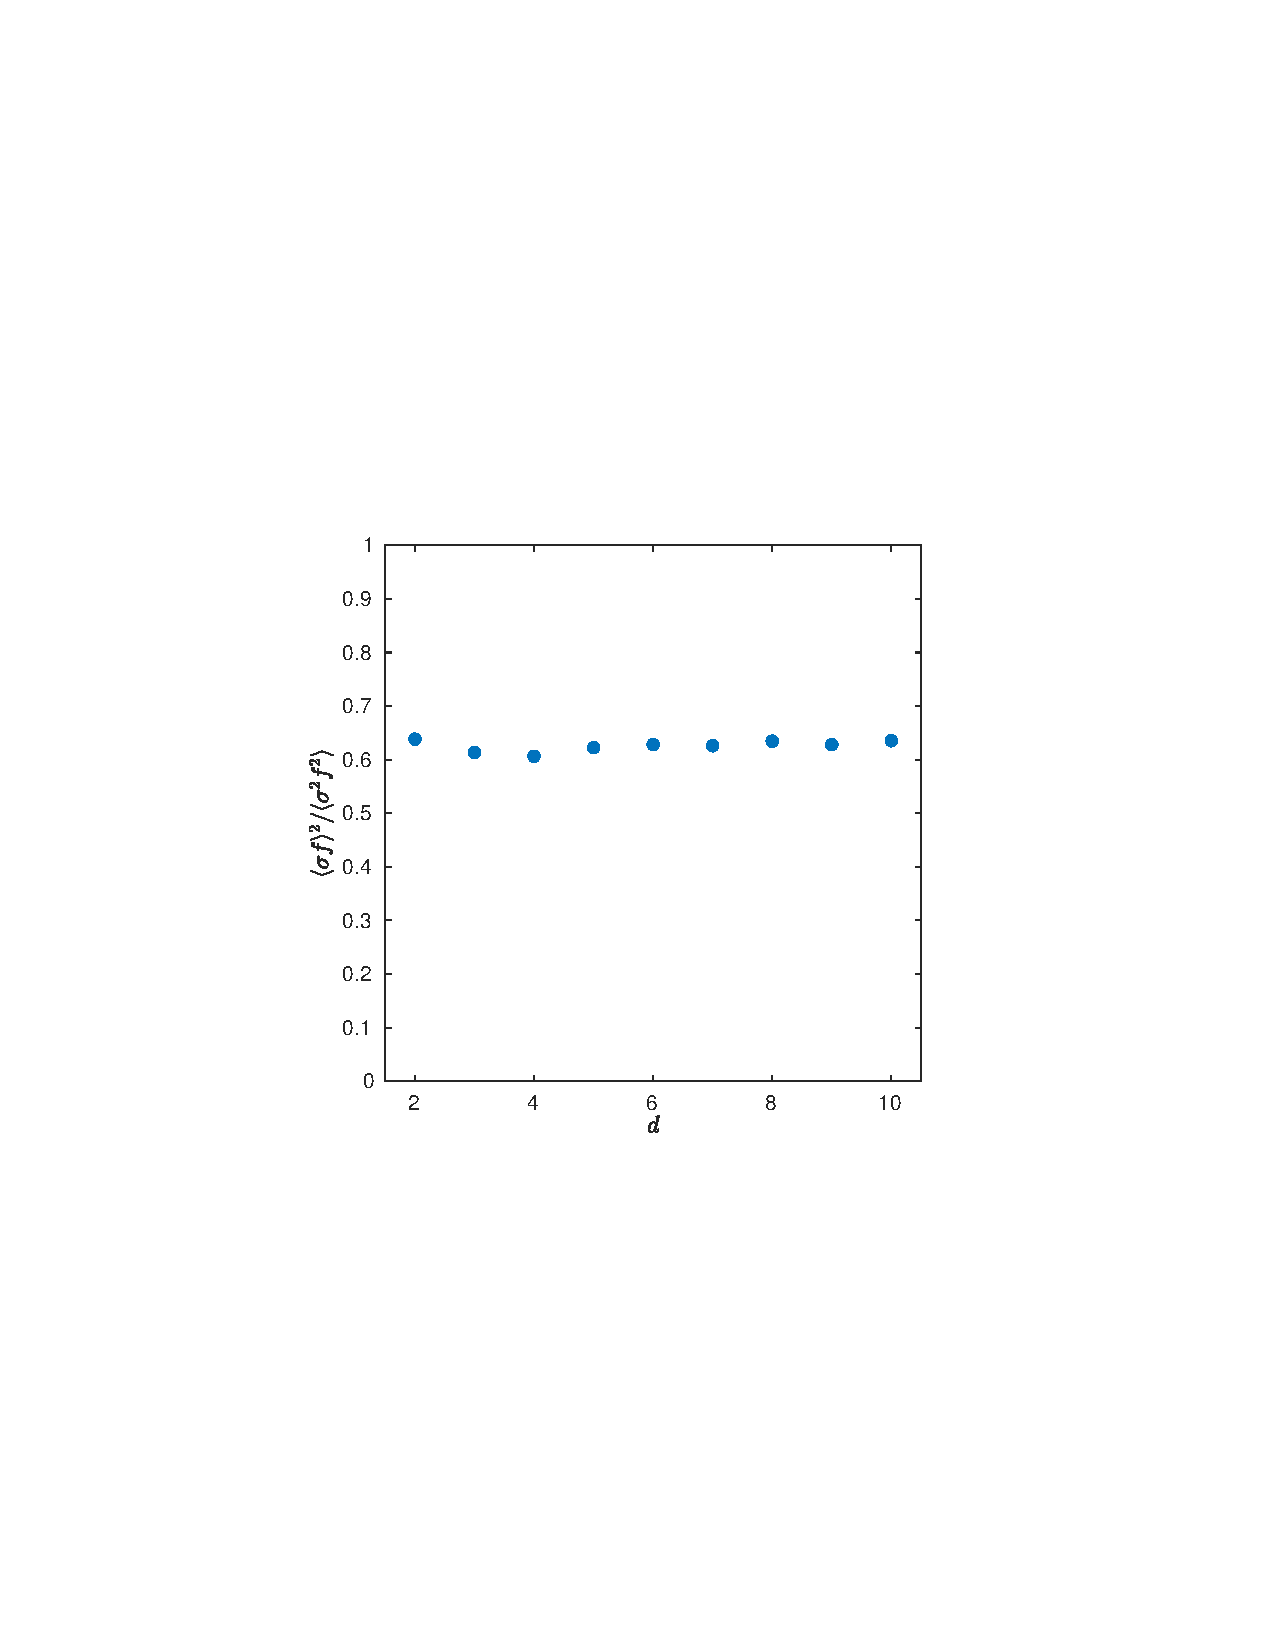
\includegraphics[width=230px, trim=133 242 168 254, clip]{excessContactsScaling/mfr.pdf}
     \caption{Dimensionless moment ratio of first and second moments of $\sigma f$ shows no dimensional dependence}
     \label{plot:mfr}
\end{figure}
\begin{figure}[h!]
     %  \end{subfigure}
%  \hfill %%
%  \begin{subfigure}[t]{0.47\columnwidth}
    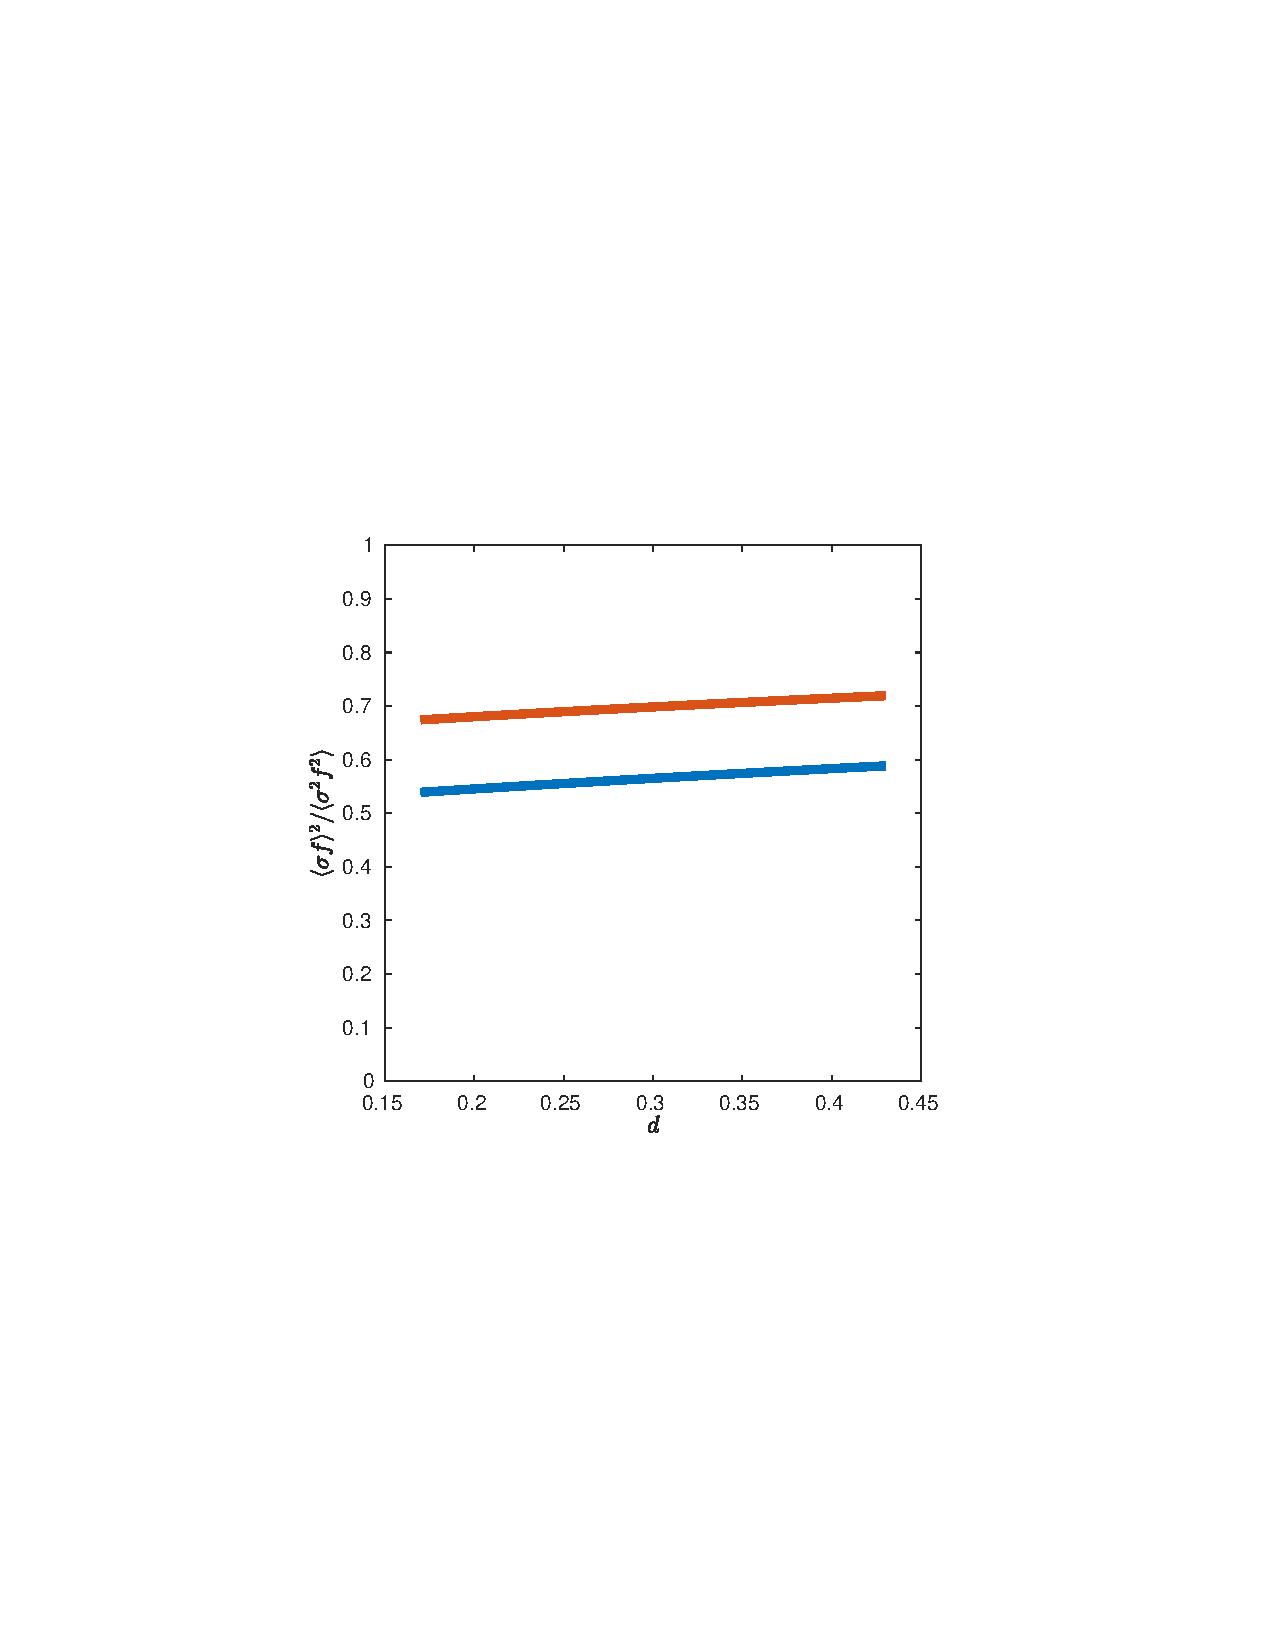
\includegraphics[width=230px, trim=143 240 163 250, clip]{excessContactsScaling/theoryMFR.pdf}
    \caption{Neither the force distribution $f^\theta e^{-f/f_0}$  (blue) nor the distribution $f^\theta e^{-f^2/f_0^2}$  (red) predicts a strong $\theta$ dependence for the relevant moment ratio}
    \label{plot:theory_mfr}
%  \end{subfigure}
\end{figure}




\subsection{Accounting for Polydispersity in Pressure vs. Packing Fraction Scaling}

To account for the case with varying spring constants we also form the matrix of inverse spring constants

\begin{equation}
k^{-1} = \frac{1}{2 \eps} \mqty(\dmat{\sigma^2_{ij},\ddots,\sigma^2_{kl}}). \label{eqn:compliance}
\end{equation}

and the projection operator onto the states of self stress

\begin{equation}
S = \sum_{i=1}^{N \Delta z} \ket{s_i}\bra{s_i}.
\end{equation}

In terms of these quantities, the bulk modulus may be written as \cite{pellegrino_structural_1993, wyart_rigidity_2005, lubensky_phonons_2015}

\begin{equation}
\pdv[2]{E}{V} = \frac{1}{V}  \bra{E} S  \left(S \left(k^{-1}\right) S \right)^{-1} S \ket{E}. \label{eqn:genf}
\end{equation}

In the one SSS approximation, we can evaluate the two projected quantities that we need to evaluate equation \ref{eqn:genf}. Equations \ref{eqn:affine} 
and \ref{eqn:sss} 
give

\begin{align}
    S \ket{E} = \bra{s_0}\ket{f} \ket{s_0}= \frac{\bra{r}\ket{f}}{d \sqrt{\bra{f}\ket{f}}}\ket{s_0} = \sqrt{Z}\frac{\langle r f \rangle}{d \sqrt{\langle f^2 \rangle}} \ket{s_0}, 
\end{align}

and equations \ref{eqn:compliance} and \ref{eqn:sss} 
give

\begin{align}
    S k^{-1} S &= \ket{s_0} \mel{s_0}{k^{-1}}{s_0} \bra{s_0} =  \ket{s_0}\frac{\langle \sigma^2 f^2 \rangle}{2 \epsilon \langle f^2 \rangle} \bra{s_0}\\
    \left(S k^{-1} S\right)^{-1} &= \ket{s_0}\frac{2 \epsilon\langle f^2 \rangle}{\langle \sigma^2 f^2 \rangle} \bra{s_0}
\end{align}

Furthermore at lowest order in $P$ we have $\ket{r} = \ket{\sigma}$, and we may assume $Z \approx d N$. Thus, equation \ref{eqn:genf} reduces to 

\begin{equation}
K = \frac{2 N \eps}{ d V}  \frac{\langle \sigma f \rangle^2}{\langle \sigma^2 f^2 \rangle},
\end{equation}

and thus via equation \ref{eqn:CisK}:

\begin{equation}
    C_{p\varphi} = \frac{2}{d} \frac{ \langle \sigma f \rangle^2}{\langle \sigma^2 f^2 \rangle}.\label{eqn:seanPredictionSupp}
\end{equation}

\subsection{Prestress Comparison}

It has recently been suggested the relationship between prestress and number of excess contacts collapses perfectly when compared across dimensions \cite{shimada_low-frequency_2019}. We define prestress $e$ as in ref. \cite{shimada_low-frequency_2019} as:
%
\begin{align}
 e = \left(d-1\right) \left\langle \frac{-V'(r_{ij})}{r_{ij}V''(r_{ij}} \right\rangle_{ij}
\end{align}
%
and expected to scale as:
%
\begin{align}
 \delta z &= C_{ze} e^\frac{1}{2} \label{sup_eqn:evsprestress}
\end{align}
%
because it is proportional to pressure near the jamming transition \cite{shimada_low-frequency_2019}. In figures \ref{plot:evsprestress} and  \ref{plot:evspcomp},, we examine the collapse of scaled excess contacts with prestress and compare it to the collapse of excess contacts scaled by the mean field prediction with pressure. In figure \ref{plot:evsprestress} we see that the collapse with prestress is not quite perfect - there is a clear upward trend. This stands in contrast to the inset of figure \ref{plot:evspcomp}, which shows $\hat{C}_{zp}$ to be nearly constant above three dimensions.


  
\begin{figure}[h!]
 %   \caption{Comparison of scaled excess contacts with pressure and prestress.}
% \label{plot:comparison}
% \begin{subfigure}[t]{0.47\columnwidth}
    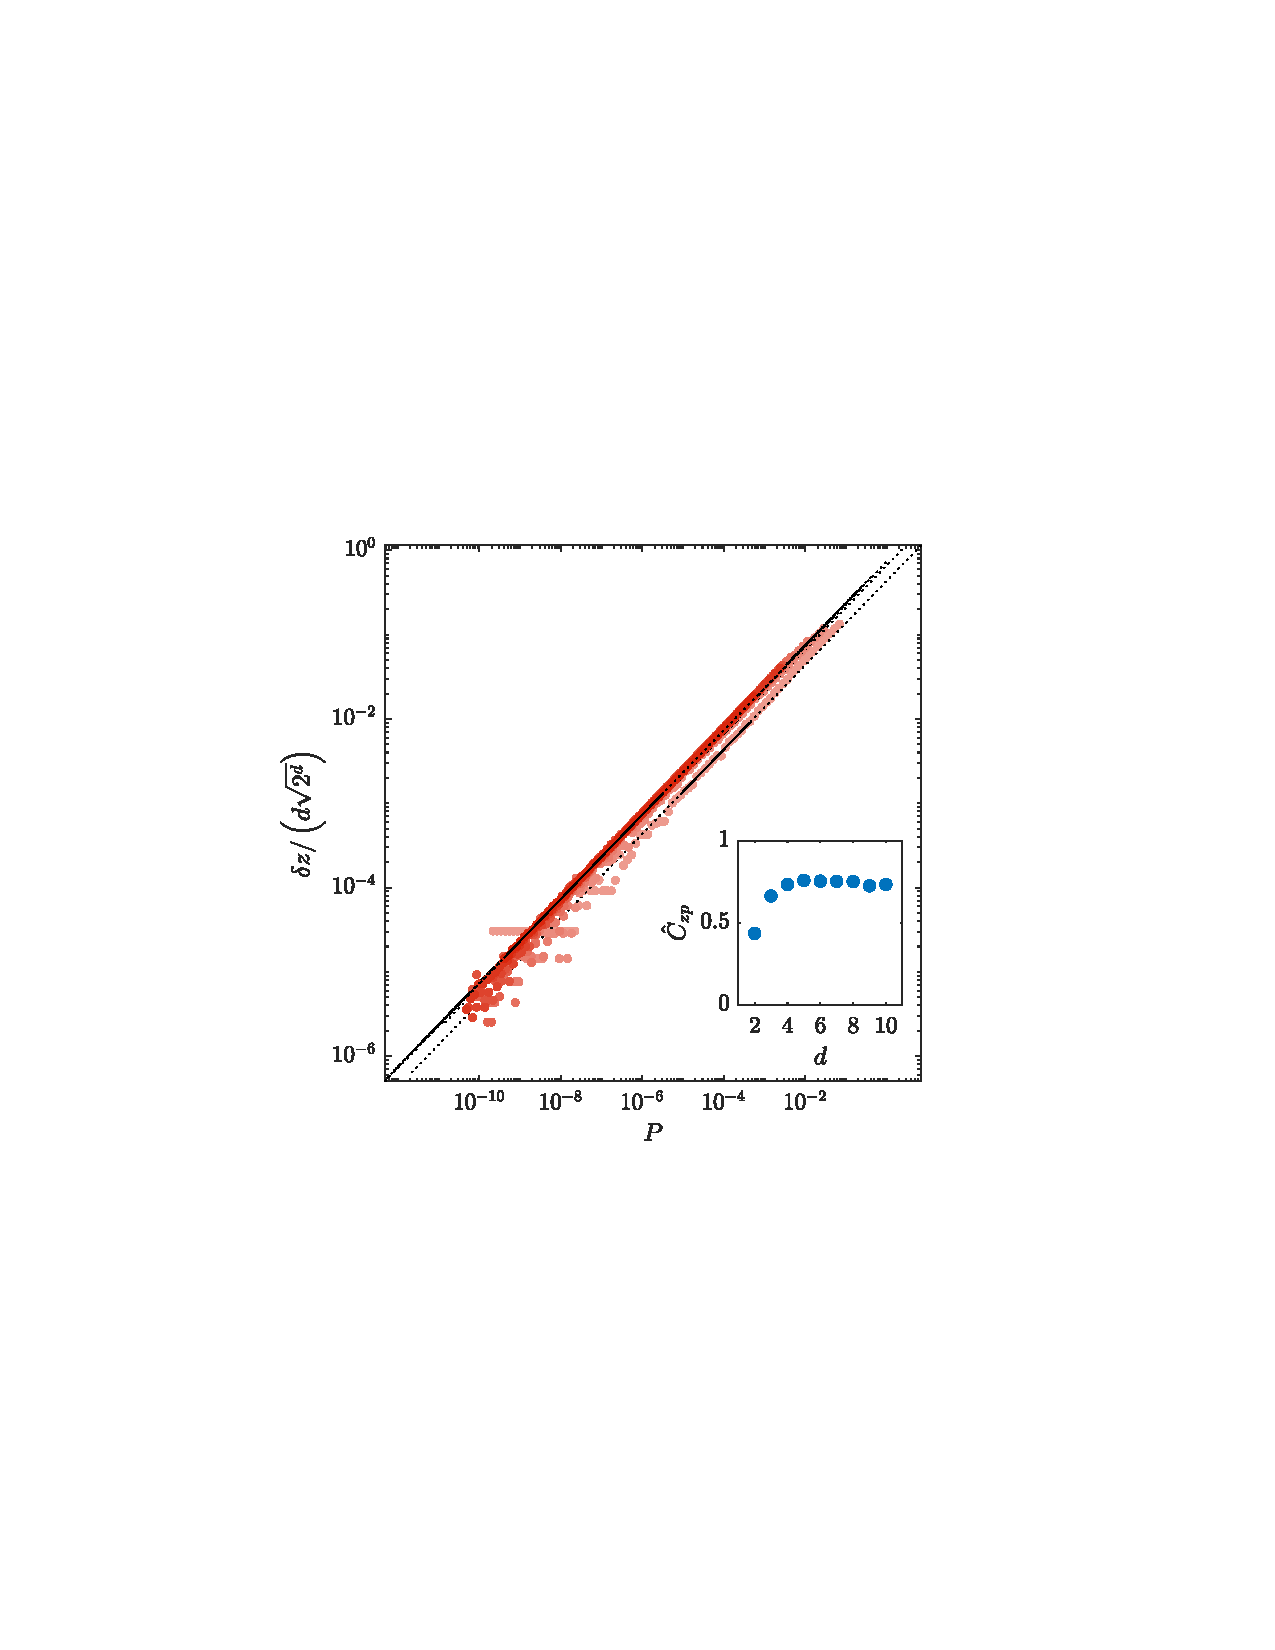
\includegraphics[width=230px, trim=133 242 168 254, clip]{excessContactsScaling/evspcomp.pdf}
   \caption{Scaled excess contacts scales with the square root of pressure as in figure \ref{plot:evsp}. 
    However, with excess contacts scaled by the expected mean field prediction, eqn. \ref{eqn:meanFieldExcessPressure},
    the data collapse onto a single line. The inset confirms the collapse, showing $\hat{C}_{zp}$ to be nearly constant.}
     \label{plot:evspcomp}
\end{figure}
\begin{figure}[h!]
%  \hfill %%
%  \begin{subfigure}[t]{0.47\columnwidth}
    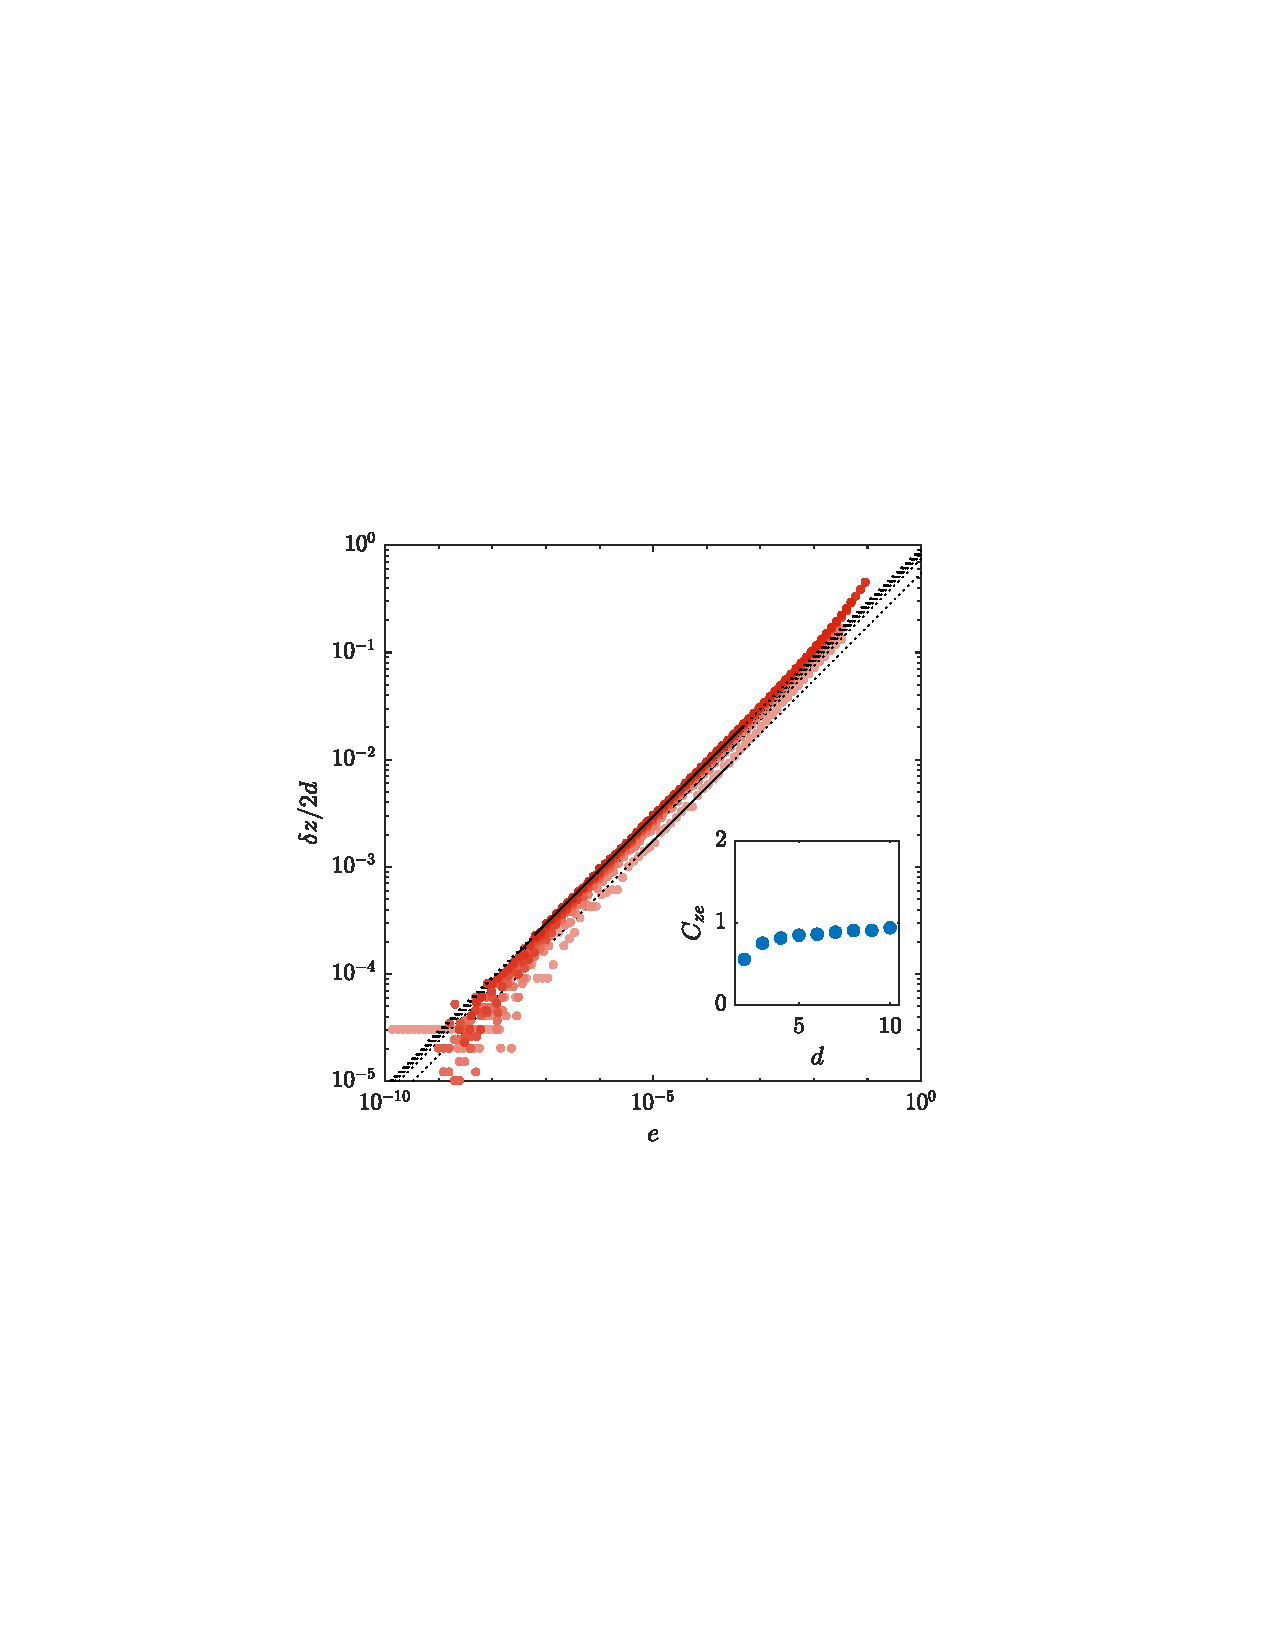
\includegraphics[width=230px, trim=143 240 163 250, clip]{excessContactsScaling/prestressvse.pdf}
    \caption{Scaled excess contacts scales with the square root of prestress for systems from $d=2$ to $d=10$. Black lines show the fits for $C_{ze}$ using eqn \ref{sup_eqn:evsprestress}. The fits ignore high and low pressure data as in figure \ref{plot:evsp}. 
    Lower inset shows the measured values of $C_{ze}$ which have a clear upward trend.}
    \label{plot:evsprestress}
%  \end{subfigure}
\end{figure}

In fact, close to jamming so that $r \approx \sigma$ and $Z \approx N d$, our dimensionless pressure $P$ as defined in equation \ref{eqn:stress_tensor_definition}  
is related to the prestress by
%
\begin{align} P &= \frac{\bar{V}_p}{\varepsilon Vd} \sum_{i,j} \mathbf{f}_{ij} \cdot \mathbf{r}_{ij} \\
  &=\frac{\bar{V}_p}{\varepsilon Vd} Z \langle f_{ij} r_{ij} \rangle_{ij} \\
  &=\frac{2 \varphi Z}{ d}  \left\langle \frac{r_{ij}}{\sigma_{ij}} \left(1 - \frac{r_{ij}}{\sigma_ij}\right) \right\rangle_{ij}\\
  &= \frac{2 \varphi Z}{d}  \left\langle \frac{- r_{ij} V'(r_{ij})}{\sigma_{ij}^2V''(r_{ij}} \right\rangle_{ij} \\
&\approx 2\frac{ \varphi_{\mathrm{J}} }{d-1} e.
\end{align}
%
Thus, our better-fitting form for the $z-P$ relationship amounts to the statement that
%
  \begin{equation}
    \frac{\Delta z}{2 d} =  \hat{C}_\varphi   \sqrt{\frac{d}{d-1}} \sqrt{e}.
  \end{equation}
%
 Thus our scaling forms agree with the statement of reference \cite{shimada_low-frequency_2019} in the infinite-$d$ limit, although we see better fit with our form in low dimensions.


%\bibliography{scaling}% Produces the bibliography via BibTeX.

%\end{document}
%yes
% ****** End of file aipsamp.tex ******



%\include{log-potential}
%\include{shear-memory}
%\include{log-potential-supplement}
%\include{shear-memroy-supplement}
%\chapter{Conclusion}

The work presented in this dissertation represents a substantial addition to the literature regarding the Force Network Ensemble for jammed amorphous systems. We have shown two new methods by which the Force Network Ensemble can be used to better understand granular systems. Additionally we have shown that jamming scaling laws can be proven from first principles without the mean field assumption, suggesting that the mean field assumption may not be necessary for understanding scaling laws in jamming.

While previous discussion of the Force Network Ensemble had been abstractly defined as a particular region in force space, our work in Chapter \ref{forceVolumeEntropyPaper} was the first to measure this space in a concrete way. Moreover, we were able to connect our measurements of the Force Network Ensemble with a bulk measurement of angoricity. In doing so we not only discovered a new quantity, $h_f$ which sets the scale of discretization for these systems, but also put the concept of angoricity on firm footing as a thermodynamic quantity. This connects thermodynamic approaches to granular materials with an underlying statistical mechanics, contributing to a complete statistical mechanical description of granular materials.

In Chapter \ref{contactBreaking} we expanded on this work, using the Force Network Ensemble to identify systems at the boundaries of available force space. From this we devised a provably correct first principles method for analytically identifying the only locations at which any contact change can occur under decompression. These force network defects are a completely new form of defect in amorphous materials and provide a framework for a ground up understanding of amorphous materials.

Despite the quantity of questions which have been answered by this work, an even greater number of interesting new questions have been raised. We hope that our approach of studying the space of allowed force configurations in granular systems serves as the foundation for future research. In particular, it would be interesting to use our strategy from Chapter \ref{contactBreaking} to predict contact breaking events in systems further from jamming via the Force Network Ensemble. While we limited our study to 2SSS systems, the same principle should apply to systems with more states of self stress. The problem becomes more challenging as the dimensionality of the space of states of self stress increases, but the same protocol can be used on a system with many states of self stress to predict not just the breakable contacts, but also all of the allowed 1SSS final configurations after decompression. Of course, since some contact breaking events are rearrangements, predictions for sequential contact breaking events will be less accurate. However, since about $86\%$ of contact network changes are stable contact network changes, we would still expect to have decent predictive power for at least a few contact breaks \cite{morse_differences_2020,tuckman_contact_2020}.

Another interesting and unexplored avenue is the search for force network defects in ultrastable systems \cite{kapteijns_fast_2019,hagh_transient_2021,ninarello_models_2017}, which have more contacts near jamming than random packings, and as such the defects may be delocalized or poorly defined. One could also attempt to modify our protocol to identify force network defects under shear rather than decompression. This would be especially interesting because the majority of the work done on soft spots has been conducted under shear, as were the recent studies which distinguished and quantified rearrangements versus stable contact network changes \cite{morse_differences_2020,tuckman_contact_2020}.

Finally, one can also envision attempting to ascertain which force network defects will be rearrangements versus stable contact network changes. This could concievably be done with machine learning, in a similar fashion to much of the soft spots literature. Perhaps only the force network defects which exist within identifiable soft spots tend to lead to rearrangements, and others tend to lead to stable contact network changes. 

In Chapter \ref{excessContactsScaling} we took highly precise measurements of jamming scaling laws to measure the prefactors to jamming scaling relations. We showed that the mean field prediction is accurate for not just scaling exponents, but even the prefactors to these scaling laws. This was quite surprising because we expect these prefactors to be nonuniversal and highly sensitive to finite dimensional corrections to mean field theory. We were additionally able to show a first principles proof for the scaling prefactor between pressure and packing fraction. This showed that the mean field assumption was not necessary for that particular relation, and suggests that other relations may similarly be proven without the need for mean field theory. This calls into question the necessity of the mean field assumption in general for glasses and jamming. In particular, is there a derivation for the prefactor between excess contacts and pressure that does not rely on the mean field assumption? Moreover, are other scaling prefactors well predicted by the mean field?  Of course, we do not expect that all useful results from the mean field may be proven without the mean field assumption - but perhaps more can be than previously thought. 


%%%APPENDICES
%%BIBILIOGRAPHY
\bibliographystyle{unsrtnat}
\bibliography{dissertation.bib}
\end{document}
